%% BioMed_Central_Tex_Template_v1.06
%%                                      %
%  bmc_article.tex            ver: 1.06 %
%                                       %

%%IMPORTANT: do not delete the first line of this template
%%It must be present to enable the BMC Submission system to
%%recognise this template!!


%%% additional documentclass options:
%  [doublespacing]
%  [linenumbers]   - put the line numbers on margins

%%% loading packages, author definitions

%\documentclass[twocolumn]{bmcart}% uncomment this for twocolumn layout and comment line below
\documentclass{bmcart}

%%% Load packages
%\usepackage{amsthm,amsmath}
%\RequirePackage{natbib}
%\RequirePackage[authoryear]{natbib}% uncomment this for author-year bibliography
%\RequirePackage{hyperref}
\usepackage[utf8]{inputenc} %unicode support
\usepackage{algorithmic}
\usepackage{rotating}
\usepackage{amsmath}
\usepackage{multirow}
\usepackage{enumerate}
\usepackage{algorithm}
\usepackage{subfigure}
%\usepackage[applemac]{inputenc} %applemac support if unicode package fails
%\usepackage[latin1]{inputenc} %UNIX support if unicode package fails


%%%%%%%%%%%%%%%%%%%%%%%%%%%%%%%%%%%%%%%%%%%%%%%%%
%%                                             %%
%%  If you wish to display your graphics for   %%
%%  your own use using includegraphic or       %%
%%  includegraphics, then comment out the      %%
%%  following two lines of code.               %%
%%  NB: These line *must* be included when     %%
%%  submitting to BMC.                         %%
%%  All figure files must be submitted as      %%
%%  separate graphics through the BMC          %%
%%  submission process, not included in the    %%
%%  submitted article.                         %%
%%                                             %%
%%%%%%%%%%%%%%%%%%%%%%%%%%%%%%%%%%%%%%%%%%%%%%%%%

%\def\includegraphic{}
%\def\includegraphics{}

%%% Put your definitions there:
\startlocaldefs
\endlocaldefs



\begin{document}
\begin{frontmatter}
\begin{fmbox}
\dochead{Research}

\title{Improving the performance of relaxed clock model in phylogenetic analysis}

\author[
   addressref={aff1},                   % id's of addresses, e.g. {aff1,aff2}
   corref={aff1},                       % id of corresponding address, if any
   %noteref={n1},                        % id's of article notes, if any
   email={alexei@cs.auckland.ac.nz}   % email address
]{\inits{}\fnm{Alexei} \snm{Drummond}}
\author[
   addressref={aff1},
   email={rzha419@aucklanduni.ac.nz}
]{\inits{}\fnm{Rong} \snm{Zhang}}

\address[id=aff1]{%                           % unique id
  \orgname{Department of Computer Science, University of Auckland}, % university, etc
  \street{Princes Street},                     %
  \postcode{1010}                                % post or zip code
  \city{Auckland},                              % city
  \cny{New Zealand}                                    % country
}

%\address[id=aff2]{%
%  \orgname{},
%  \street{},
%  \postcode{}
%  \city{},
%  \cny{}
%}

%\begin{artnotes}
%%\note{Sample of title note}     % note to the article
%\note[id=n1]{Equal contributor} % note, connected to author
%\end{artnotes}

\end{fmbox}% comment this for two column layout

%%%%%%%%%%%%%%%%%%%%%%%%%%%%%%%%%%%%%%%%%%%%%%
%%                                          %%
%% The Abstract begins here                 %%
%%                                          %%
%% Please refer to the Instructions for     %%
%% authors on http://www.biomedcentral.com  %%
%% and include the section headings         %%
%% accordingly for your article type.       %%
%%                                          %%
%%%%%%%%%%%%%%%%%%%%%%%%%%%%%%%%%%%%%%%%%%%%%%
\begin{abstractbox}
\begin{abstract}
Bayesian MCMC plays an important role in phylogenetic analysis. However, due the huge amount of phylogenetic data, the efficiency becomes a great problem. Based on uncorrelated relaxed clock model, this paper introduces a new operator to propose evolutionary rates and divergence times while maintaining the genetic distance constant. Specifically, the proposed operator deals with three rates when changing the node time for an internal node. For the root of a phylogenetic tree, there are three strategies discussed, including Simple Distance, Small Pulley and Big Pulley. It is noticed that Big Pulley is able to change the tree topology, which enables the operator to sample all the possible trees under an unrooted tree.  To validate the effectiveness, experiments have been performed by implementing the operator in BEAST2 software. The results prove that the proposed operator is able to improve the performance by giving better estimation and less running time.
\end{abstract}

\begin{keyword}
\kwd{Bayesian MCMC}
\kwd{Operator}
\kwd{Phylogenetic trees}
\kwd{Genetic distances}
\kwd{Divergence times}
\kwd{Evolutionary rates}
\end{keyword}

% MSC classifications codes, if any
%\begin{keyword}[class=AMS]
%\kwd[Primary ]{}
%\kwd{}
%\kwd[; secondary ]{}
%\end{keyword}

\end{abstractbox}
%
%\end{fmbox}% uncomment this for twcolumn layout
\end{frontmatter}

%%%%%%%%%%%%%%%%%%%%%%%%%%%%%%%%%%%%%%%%%%%%%%
%%                                          %%
%% The Main Body begins here                %%
%%%%%%%%%%%%%%%%%%%%%%%%%%%%%%%%%%%%%%%%%%%%%%

%%%%%%%%%%%%%%%%
\section*{Introduction}
Phylogenetics has attracted much research interest over the years. More and more scientists are becoming keen to discover the evolutionary history of life, such as birds \cite{hackett2008phylogenomic}, primates \cite{szalay2013evolutionary}, grasses \cite{kellogg2001evolutionary} and so on \cite{sawabe2007inferring,garnery1992evolutionary}. One fundamental concept in phylogenetics is a graph model that shows the relationships among species and organisms, which is called a phylogenetic tree. The main task for phylogenetic analysis is aimed at inferring the phylogenies by constructing the phylogenetic trees. Until now, a lot of methods have already been proposed and a majority of them have been implemented in the computer softwares, such as BEAST2 \cite{drummond2007beast, bouckaert2014beast} , MRBAYES \cite{huelsenbeck2001mrbayes} and APE \cite{paradis2004ape}.

Traditional methods for constructing phylogenetic trees are based on a distance matrix that is obtained by sequence alignment, after biologists extract DNA from organisms. In the last few decades, more advanced techniques have been developed to reconstruct phylogenetic trees, due to the development of statistics and computer science. One popular research area called Bayesian phylogenetics puts an emphasis on a sampling process to construct the phylogenetic tree, in which the methods based on Markov Chain Monte Carlo (MCMC) provide a computational tool for sampling problems. For example, Yang and Rannala presented a Bayesian framework that includes the specified prior for phylogenies and ancestral speciation times, and the posterior probabilities of phylogenies to be inferred as the maximum posterior probability (MAP) tree \cite{yang1997bayesian}. Specifically, Monte Carlo integration is used to integrate over the ancestral speciation times for particular trees and a MCMC method is used to sample a set of trees with probabilities. Based on this framework, much attention has been paid to estimating the divergence times \cite{rannala2003bayes,yang2003comparison,reis2011approximate}.

For phylogenetic analysis based on Bayesian MCMC, the efficiency of a sampling method is always the main issue that should be carefully dealt with. In particular, the calculation of the phylogenetic likelihood is a large burden of the efficiency. Hence, some researchers have tried to improve the likelihood calculations, such as detection of repeating sites \cite{kobert2017efficient}. On the other hand, in MCMC methods, the operators that propose a new state based on the current state also have a leading influence on the overall performance. As is discussed by Lakner et al., the major limitation in Bayesian MCMC analysis of phylogeny lies in the efficiency with which operators sample the tree space \cite{lakner2008efficiency}. So far, there have been already many different kinds of operators proposed. According to the work in Ref. \cite{hohna2011guided}, the two common operators, i.e. prune-and-regraft and subtree-swap, both contribute to a tree with low likelihood since they propose a new tree by random movement of the current tree. So the authors introduced two new operators by proposing a state from a discrete set of possible proposals and narrowing the proposal distribution to the more likely proposals. Their experimental results proved that the two operator have faster average run time and more accurate predictability.

Nevertheless, it is acknowledged that a faster and more reliable performance is also dependent on a good mixture of operators and different operators may be applicable for different objects. In this paper, a novel operator is proposed in the case where genetic distances are constant. Namely, the proposed operator is used to change the divergence times of nodes and evolutionary rates on the branches at the same time without changing the genetic distances, so that the likelihood of the phylogenetic tree remains unchanged. According to a series of simulations and experiments, it is concluded that by using the proposed operator, the tree will be sampled more efficiently in the MCMC runs.

The following of this paper is constructed as follows: Section 2 gives some preliminary theories of the work related to this paper. Section 3 introduces the proposed operator, which includes the mechanism for internal nodes and 3 different strategies for the root. The experiments and discussions are detailed in the 4th section to validate the efficiency of the proposed operator. Section 5 ends the paper with a short conclusion.
\section*{Prelimiaries}
\subsection*{Bayesian MCMC}
Eq.(\ref{bayes}) shows a basic Bayesian framework for phylogenetic analysis. It consists of prior distributions for the tree and parameters of interest $\Pr (g) $ and $\Pr (\Phi )$, a phylogenetic likelihood $\Pr (D|g,\Phi )$ and the posterior distribution $f(g,\Phi |D)$ that is to be inferred. So from a Bayesian perspective, the biological data, phylogenetic trees and all the parameters in the model exist in the form of a distribution and are related by the Bayes' formula. As a result, it is able to combine different models that describe various biological and evolutionary process at the same time.
\begin{eqnarray}\label{bayes}
f(g,\Phi |D) = \frac{{\Pr (D|g,\Phi ) \times \Pr (g) \times \Pr (\Phi )}}{{\Pr (D)}}
\end{eqnarray}
, where $g$ denotes the phylogenetic tree, $\Phi$ is a set of parameters and $D$ represents the data available.

Moreover, due to the huge amount of data and the marginal likelihood being difficulty to calculate, Markov Chain Monte Carlo (MCMC) algorithms are adopted to get samples from the posterior distribution.
\subsection*{Tree proposals}
The term ``operator" used in this paper is defined as the tree proposal in Bayesian MCMC to propose a new state that is only dependent on the current state.

Generally, some classical operators can satisfy most sampling requirements, such as a random walk operator which proposes a new state by adding a random number, and a scale operator which multiplies the current state with a scale factor. But they are suitable for working on a single parameter or a set of parameters, such as population size. To make a proposal about the tree topology, it is also necessary to include other operators, such as subtree slide operator, swap operator narrow operator and so on. On top of this, there are also some extended operators available to help give the better performance. For instance, the prune-and-regraft operator selects a random subtree and reattaches the subtree at a new random branch. And the subtree-swap operator exchanges two random subtended subtrees.

What matters for developing an operator is that the proposal should be reversible. As is discussed in Green's paper \cite{green1995reversible}, the constructed Markov transition kernel $P(x,dx')$ should satisfy the detailed balance, as is shown by Eq.(\ref{balance}). Consequently, the probability that the operator propose a new state from the current state is required to be equal to the probability that the proposed state goes back to current state. Therefore, in Eq.(\ref{Ratio}), to ensure the detailed balance in the MCMC chain, a ratio ${q(x',dx)}/{q(x,dx')}$ should always be included in the probability $\alpha(x,x')$ that the proposal made by the operator is accepted, which is defined as \textit{Hasgtings ratio}.
\begin{equation}\label{balance}
\int_A {\int_B {\pi (dx)P(x,dx')} }  = \int_B {\int_A {\pi (dx')P(x',dx)} }
\end{equation}
, where ${\pi (dx)}$ is the target distribution, $A$ and $B$ are Borel sets in parameter space $\varphi$.
\begin{equation}\label{Ratio}
{\alpha}(x,x') = \min \left\{ {1,\frac{{\pi (dx'){q}(x',dx)}}{{\pi (dx){q}(x,dx')}}} \right\}
\end{equation}
\subsection*{Uncorrelated relaxed clock model}
A clock model is used to model how rates evolve along branches in the phylogenetic tree, so that a time tree can reconcile with the genetic distances between sequences described by a substitution model. For example, a strict clock model assumes evolution rates to be the same at every branch. However, a relaxed clock model allows rates to vary across lineages so that better estimates of divergence times can be obtained. As a incomplete way of relaxing, a random local clock model only allows rates to be different within a subregion of the tree.

In this paper, the proposed operator is based on an uncorrelated relaxed model, where the rates vary and follow a certain distribution. As is detailed in Ref.\cite{drummond2006relaxed}, uncorrelated rates indicate that the rate on each branch is identically distributed and will be independently drawn from a certain distribution such as a log-normal distribution. As a result, the rates can change faster than making a slight move over multiple adjoining branches.
\section*{The proposed operator}
We define the proposed operator as ConstantDistance Operator (cons for abbreviation).The flow chart of the proposed operators is shown in Fig.\ref{flowchart}. In a phylogenetic tree, the node operated on is denoted by \textbf{X}. And the proposed operator works differently on the internal nodes and the root of the tree. The details of the operations are introduced step by step as follows.
\subsection*{The internal node operator}
Fig.\ref{internalnodes} represents the tree (or subtree of a phylogenetic tree) with the node \textbf{X}, which is randomly selected among the internal nodes, as well as its parental node and two child nodes. The original tree on the left is denoted by Tree. And the following 5 steps will propose a new tree, denoted by Tree', on the right.

\emph{Step 1} Get the parent node and two child nodes of \textbf{X}, denoted by \textbf{P}, \textbf{Ch1} and \textbf{Ch2} respectively.

\emph{Step 2} Get the nodes times of \textbf{X}, \textbf{P}, \textbf{Ch1} and \textbf{Ch2} , denoted by $t_X$, $t_P$, $t_1$, $t_2$, as well as the rates on the branches above the nodes, denoted by $r_i$, $r_j$, $r_k$.

\emph{Step 3} Propose a new node time for \textbf{X} by ${t_X}' = {t_X} + a$, where $a$ follows a Uniform distribution with a symmetric window size, i.e. $a \sim Uniform[ - w, + w]$. Make sure that the proposed time is valid, i.e. $\max \{ {t_1},{t_2}\}  < {t_X}' < {t_P}$ holds.

\emph{Step 4} Propose new rates by using Eq.(\ref{int_rate}).
\begin{equation}
 \label{int_rate}
{r_i}' = \frac{{r_i} \times ({{t_P} - {t_X}})}{{{t_P} - {t_X}'}}\\
{r_j}' = \frac{{{r_j} \times ({{t_X} - {t_1}})}}{{{t_X}' - {t_1}}}\\
{r_k}' = \frac{{{r_k} \times ({{t_X} - {t_2}})}}{{{t_X}' - {t_2}}}
 \end{equation}

\emph{Step 5} Return the $HastingsRatio$.

\subsection*{The root operator}
For the root of the tree, there are three strategies to propose the new rates and node times. To be more specific, Simple Distance is a way of proposing a new root time only. Considering the genetic distance, Small Pulley makes changes for branches on each side of the root. Moreover, under the constraint that the unrooted tree is fixed, Big Pulley proposes a new tree topology by rearranging the root.  Details are discussed below
\subsubsection*{Simple Distance}
Fig.\ref{simpledistance} shows the trees that are rooted at the selected node $X$. The initial tree in Fig.\ref{simpledistance}(a) represents the current state, which is denoted by Tree. Inspired by how the operations on internal nodes, we will use the following steps to propose a new tree, denoted by Tree', and keep the genetic distances $d_i$ and $d_x$ constant at the same time, as is shown in Fig.\ref{simpledistance}(b).

\emph{Step 1} Get the child nodes of the root \textbf{X}, denoted by \textbf{son} and \textbf{dau}. Their corresponding node times and rates are $t_X$, $t_j$, $t_k$ and $r_i$, $r_x$.

\emph{Step 2} Propose a new node time for the root \textbf{X} by \textbf{X} by ${t_X}' = {t_X} + a$, where $a \sim Uniform[ - w, + w]$. Make sure that ${t_X}' > \max \{ {t_j},{t_k}\} $ holds.

\emph{Step 3} Propose new rates for branches on each side of the root by using Eq.(\ref{sim_rate}).
\begin{equation}
\label{sim_rate}
{r_i}' = \frac{{{r_i} \times ({{t_X} - {t_j}})}}{{{t_X}' - {t_j}}}\\
{r_x}' = \frac{{{r_x} \times ({{t_X} - {t_k}})}}{{{t_X}' - {t_k}}}
 \end{equation}

\emph{Step 4} Return the $HastingsRatio$.
\subsubsection*{Small Pulley}
Different from Simple Distance, a new genetic distance of branch on one side of the root is proposed in Small Pulley. As is indicated in Fig.\ref{simpledistance}, Small Pulley proposed a new tree in Fig.\ref{simpledistance}(c), based on the current state in Fig.\ref{simpledistance}(a). In order to remain the total genetic distance of $d_i$ and $d_x$ unchanged, once ${d_i}'$ is proposed, $d_x$ will be adjusted by ${d_x}'$ simultaneously. The detailed process includes the following four steps.

\emph{Step 1} Get the child nodes of the root \textbf{X}, denoted by \textbf{son} and \textbf{dau}. Their corresponding node times and rates are $t_X$, $t_j$, $t_k$ and $r_i$, $r_x$. So the genetic distances can be calculated according to Eq.(\ref{sma1_dis}).
\begin{equation}
\label{sma1_dis}
{d_i}' = {r_i} \times ({{t_X} - {t_j}})\\
D = {d_i} + {r_x} \times ({{t_X} - {t_k}})
 \end{equation}

\emph{Step 2} Propose a new genetic distance for $d_i$ by adding a random number that follows a Uniform distribution, i.e.  ${d_i}' = {d_i} + b$, where $b \sim Uniform[ - v, + v]$. Make sure that $0 < {d_i}' < D$ holds, where $D = {d_i} + {d_x}$.

\emph{Step 3} Propose new rates for branches on each side of the root by using Eq.(\ref{sma1_rate}).
\begin{equation}
\label{sma1_rate}
{r_i}' = \frac{{{d_i}'}}{{{t_X} - {t_j}}}\\
{r_x}' = \frac{{D - {d_i}'}}{{{t_X} - {t_k}}}
 \end{equation}

\emph{Step 4} Return the $HastingsRatio$.
\subsubsection*{Big Pulley}
Big Pulley is used to sample the rates and times from a fixed unrooted tree so that the genetic distances among taxon are constant, which means the location of the root will be rearranged.

Firstly, a method called \textit{Exchange (Node1,Node2)} is designed to propose a new tree topology in this circumstances. For the tree in Fig.\ref{exchangemethod}, once the method \textit{Exchange (\textbf{B},\textbf{C})} is called, the following operations will be performed to proposed a new tree, as is shown on the right in the figure.
\begin{enumerate} [(1)]
\item Propose ${d_i}'$ by ${d_i}' = {d_i} + b$, where $b \sim Uniform[ - v, + v]$. Make sure that $0 < {d_i}' < D$ holds, where $D = {d_i} + {d_x}$.
\item Exchange the node \textbf{B} and \textbf{C} by pruning and grafting, i.e. cutting \textbf{B} (\textbf{C}) at its original position and attaching it to the original position of \textbf{C} (\textbf{B}).
\item To maintain the genetic distances $d_{AB}$, $d_{AC}$ and $d_{BC}$ constant, the distances on the other three branches $d_j$, $d_k$ and $d_x$ will be adjusted by using Eq.(\ref{big_dis}).
% \begin{subequations}\label{big_dis}
%  \begin{equation}
%{d_j}' = {d_j}
%  \end{equation}
%  \begin{equation}
%{d_k}' = {d_k} - {d_i}'
%  \end{equation}
%    \begin{equation}
%{d_x}' = {d_x} + {d_i}
%  \end{equation}
%\end{subequations}
\begin{equation}\label{big_dis}
{d_j}' = {d_j}\\
{d_k}' = {d_k} - {d_i}'\\
{d_x}' = {d_x} + {d_i}
\end{equation}
\end{enumerate}

As can be seen from the above descriptions, the method \textit{Exchange (Node1,Node2)} is actually aimed at swapping two nodes and reassigning distances on the four branches.

Secondly, before applying this method in Big Pulley, there are two different tree shapes to take into consideration. In Fig.\ref{treeshape}, a symmetric tree is shown on the left, in which both the child nodes of the root have child nodes. But in an asymmetric tree, only one of the child nodes of the root has child nodes below it, which means the other child node of the root is a leaf node. Hence, Big Pulley also differs when it works on a symmetric and asymmetric tree. The corresponding operations are detailed in the following two parts.
\paragraph*{Symmetric tree shape}

For the symmetric tree in Fig.\ref{treeshape}, the operations are illustrated in Fig.\ref{symmetric}, after which one of the four possible trees will be proposed.

\emph{Step 1} Get the child nodes of the root \textbf{X}, denoted by \textbf{son} and \textbf{dau}. And the child nodes below them are denoted by $Ch1$, $Ch2$, $Ch3$ and $Ch4$. Correspondingly, the node times are denoted by $t_X$, $t_j$, $t_k$.

\emph{Step 2} Propose a new node time for the root \textbf{X} by \textbf{X} by ${t_X}' = {t_X} + a$, where $a \sim Uniform[ - w, + w]$.

\emph{Step 3} Propose a new node time either for \textbf{son} or \textbf{dau}. And apply the method using \textbf{dau} and either child node of \textbf{son}.
\begin{itemize}
\item With 0.5 probability to pick \textbf{son} and propose a new node time by ${t_j}' = {t_j} + {a_1}$, where ${a_1} \sim Uniform[ - w, + w]$. Make sure that ${t_k} < {t_j}' < {t_X}'$ holds. Then, there are two options to apply the method, i.e.

\textcircled1: With 0.5 probability to \textit{Exchange (\textbf{Ch1} and \textbf{dau})}

\textcircled2: With 0.5 probability to \textit{Exchange (\textbf{Ch2} and \textbf{dau})}

\item With 0.5 probability to pick \textbf{dau} and propose a new node time by ${t_k}' = {t_k} + {a_2}$, where ${a_2} \sim Uniform[ - w, + w]$. Make sure that ${t_j} < {t_k}' < {t_X}'$ holds. Similarly, there are two options to apply the method, i.e.

\textcircled3: With 0.5 probability to \textit{Exchange (\textbf{Ch3} and \textbf{son})}

\textcircled4: With 0.5 probability to \textit{Exchange (\textbf{Ch4} and \textbf{son})}
\end{itemize}

\emph{Step 4}  Update the rates using the adjusted genetic distances divided by the proposed node times.

\emph{Step 5} Return the Hastings Ratio
\paragraph*{Asymmetric tree shape}

How to operate on the asymmetric tree in Fig.\ref{treeshape} is illustrated Fig.\ref{asymmetric}, in which there are three possible trees.

\emph{Step 1} Get the older child of the root, denoted by \textbf{O}, and the younger child of the root is denoted by \textbf{Y}. The node times of the root and its child nodes are denoted by ${t_O}$, ${t_{O1}}$ and ${t_{O2}}$.

\emph{Step 2} Propose a new node time for \textbf{O} by ${t_O}' = {t_O} + {a_3}$, where ${a_3} \sim Uniform[ - w, + w]$.

\emph{Step 3} Apply the method using \textbf{Y} and either child nodes of \textbf{O}, which is dependent on ${t_O}'$.
\begin{itemize}
\item if ${t_O}'$ satisfies ${t_O}' > \max \{ {t_{O1}},{t_{O2}}\} $ or ${t_{O1}} = {t_{O2}}$, then there are two options, i.e.

\textcircled5: With 0.5 Probability to \textit{Exchange (\textbf{O1} and \textbf{Y})}

\textcircled6: With 0.5 Probability to \textit{Exchange (\textbf{O2} and \textbf{Y})}
\item if ${t_O}'$ satisfies $\min \{ {t_{O1}},{t_{O2}}\}  < {t_O}' < \max \{ {t_{O1}},{t_{O2}}\} $, then there is only one option, i.e.

\textcircled7: Exchange the older child of \textbf{O} and \textbf{Y}.  In the example here, we apply \textit{Exchange (\textbf{O1}  and \textbf{Y})}.
\end{itemize}

\emph{Step 4}  Update the rates using the adjusted genetic distances divided by the proposed node times.

\emph{Step 5} Return the Hastings Ratio
\paragraph*{Hastings Ratio}
Algorithm \ref{alg1}.
\begin{algorithm}
\caption{Return HastingsRatio for Big pulley}
\label{alg1}
\begin{algorithmic}[1]
\IF{the node that has been exchanged with \textbf{dau} or \textbf{dau} has child nodes}
\STATE $\alpha  = \beta  = 0.25$
\ELSIF{${t_R} > {t_L}$}
\STATE $\alpha  = 1,\beta  = 0.5$
\ELSIF{${t_R} < {t_L}$}
\STATE $\alpha  = 0.5,\beta  = 1$
\ELSIF{${t_R} = {t_L}$}
\STATE $\alpha  = \beta  = 1$
\ENDIF
\IF{the node that has been exchanged with \textbf{O} has child nodes}
\STATE $\gamma  = 0.25$
\ELSE
\STATE $\gamma  = 0.5$
\ENDIF
\FOR{\textcircled1 \textcircled2}
\STATE Return $HastingsRatio = \frac{\alpha }{{0.25}}$
\ENDFOR
\FOR{\textcircled3 \textcircled4}
\STATE Return $HastingsRatio = \frac{\beta }{{0.25}}$
\ENDFOR
\FOR{\textcircled5 \textcircled6}
\STATE Return $HastingsRatio = \frac{\gamma }{{0.5}}$
\ENDFOR
\FOR{\textcircled7}
\STATE Return $HastingsRatio = \frac{{0.25}}{1}$
\ENDFOR
\end{algorithmic}
\end{algorithm}
\section*{Experimental results and analysis}
In this section, a series of experiments are conducted, together with some analysis and discussions, to validate the effectiveness and efficiency of the proposed operator. Specifically, by sampling from the prior distributions, in which no alignments are involved, the correctness of the operator is proved. After the well-calibrated simulation study, it turns out that the operator is able to work properly with other operators and sample the simulated data correctly. Besides, comparing ESS and running time, it is demonstrated that the performance is improved when the proposed operator is included.

\subsection*{Sample from the prior}
In Fig.\ref{sampleprior}, a tree with three taxa $A$, $B$ and $C$  is used as a small example in this experiment, where Tree1 is set as the initial state. First of all, a LogNormal distribution is set as the rate prior, given by Eq.(\ref{rateprior}).
\begin{equation}\label{rateprior}
r = [{r_i}\quad{r_j}\quad{r_k}\quad{r_x}] \sim LogNormal(M = -3, S = 0.5)
\end{equation}

Additionally, a Coalescent model with constant population size ($N=0.3$) is used to describe the tree prior. Hence, for a tree with 3 taxa, the probability of node times given the tree is calculated by Eq.(\ref{treeprior}).
\begin{equation}\label{treeprior}
P({t_E},{t_D}) = (\frac{1}{N} \times {e^{ - \frac{1}{N}({t_E} - {t_D})}}) \times (\frac{1}{N} \times {e^{ - \frac{3}{N}{t_D}}})
\end{equation}

After the prior is specified, the distribution to sample can be exactly known, since the samples are from the prior distributions. In other words, as the rates are the functions of its genetic distance and times, the joint distribution to sample can be represented by Eq.(\ref{integration}).
\begin{equation}\label{integration}
\begin{aligned}
P(r,t) &= P({t_E},{t_D}) \times P({r_i}) \times P({r_j}) \times P({r_k}) \times P({r_x}) \\&= P({t_E},{t_D}) \times P(\frac{{{d_i}}}{{\Delta t1}}) \times P(\frac{{{d_j}}}{{\Delta t2}}) \times P(\frac{{{d_k}}}{{\Delta t3}}) \times P(\frac{{{d_x}}}{{\Delta t4}})
\end{aligned}
\end{equation}
, where ${\Delta t}$ represents the time duration along the corresponding branch, and $P({.})$ is the probability of the LogNormal distribution. Therefore, the whole probability can be obtained by conducting numerical integration on Eq.(\ref{integration}), which shows the average over all the possible values of parameters.
\subsubsection*{Test the operator on internal nodes}
The genetic distances, node times and rates for the Tree1 in Fig.\ref{sampleprior} are given in Table \ref{ini_inter}. To test roundly, two scenarios are considered. In each scenario, the genetic distances are fixed, the node time $t_D$ starts from the initial value and is changed by the operator during the sampling process, so that node D moves between node A and E. Besides, to make sure that the result is robust, two different MCMC chain lengths are performed in each scenario.

The mean, mean error and the standard deviation of the sampled distribution are summarised in Table \ref{res_inter}. By using Eq.(\ref{integration1}), the actual joint distribution is obtained according to Eq.(\ref{integration}), and is used to evaluate the results, which is also included in Table \ref{res_inter}. Besides, the histograms of MCMC samples, as well as the curves of the numerical integration of Eq.(\ref{integration1}), are shown in Fig.\ref{res_int}. It can be seen that the red curves well fit the histograms, and the mean values and standard deviations are consistent, which makes it safe to conclude that the proposed operators works properly on the internal nodes.
\begin{equation}
\label{integration1}
P(r,{t_D}) = \int_{{t_D} = 0}^{{t_E}} {P({t_E},{t_D}) \times P(\frac{{{d_j}}}{{{t_D}}}) \times P(\frac{{{d_k}}}{{{t_D}}}) \times P(\frac{{{d_i}}}{{{t_E} - {t_D}}}) \times P(\frac{{{d_x}}}{{{t_E}}}){d_{t_D}}}
\end{equation}
\subsubsection*{Test the operator on root}
Still starting from Tree1 in Fig.\ref{sampleprior}, the initial settings for testing the root are given in Table \ref{ini_sim}. And the three strategies are tested separately in the following parts.

\paragraph*{Using Simple Distance}

The root time $t_E$ is sampled by Simple Distance, which ranges from 1 to positive infinity theoretically. Namely, all the genetic distances and the node time $t_D$  are fixed. Hence, similar to Eq.(\ref{integration1}), the sampled distribution of $t_E$ can be obtained by Eq.(\ref{integration2}).
\begin{equation}
\label{integration2}
P(r,{t_E}) = \int_{{t_E} = 1}^{ + \infty } {P({t_E},{t_D}) \times P(\frac{{{d_j}}}{{{t_D}}}) \times P(\frac{{{d_k}}}{{{t_D}}}) \times P(\frac{{{d_i}}}{{{t_E} - {t_D}}}) \times P(\frac{{{d_x}}}{{{t_E}}}){d_{t_E}}}
\end{equation}

The results are given in Table \ref{res_sma} and Fig.\ref{Fig.sub.5}. Obviously, the mean and the standard deviation are close enough, which confirms that the two distribution are the same. Thus, Simple Distance is proved to be correct.

\paragraph*{Using Small Pulley}

Although both ${d_x}$ and ${d_i}$ are changed during the sampling process when using Small Pulley, the sum of ${d_x}$ and ${d_i}$ are kept 0.67 in this test, as is shown in Table \ref{ini_sim}. To make it simple to represent, only ${d_i}$ is compared in this subsection.

Then, based on Eq.(\ref{integration}), the exact distribution of ${d_i}$ can be obtained by Eq.(\ref{integration3}), which is compared with the sampled distribution in Table \ref{res_sma} and Fig.\ref{Fig.sub.6}. Even though there exist some errors, the sampled parameters can be considered to follow the same distribution. So the Small Pulley also is able to provide the correct samples.
\begin{equation}\label{integration3}
P(r,{d_i}) = \int_{{d_i} = 1}^{0.67} {P({t_E},{t_D}) \times P(\frac{{{d_j}}}{{{t_D}}}) \times P(\frac{{{d_k}}}{{{t_D}}}) \times P(\frac{{{d_i}}}{{{t_E} - {t_D}}}) \times P(\frac{{0.67 - {d_i}}}{{{t_E}}}){d_{d_i}}}
\end{equation}

\paragraph*{Using Big Pulley}

For Tree1 in Fig.\ref{sampleprior} with tree taxa, a new tree, together with the root time $t_E$ and it older child node time $t_D$, as well as a genetic distance $d_i$, is proposed by Big Pulley. In this case, the initial state Tree1 will either go to Tree2 or Tree3, as is shown in Fig.\ref{sampleprior}.  According to the initial settings in Table \ref{ini_sim}, the genetic distances remain unchanged during the process, i.e. $d_{AB} = 1$, $d_{AC}  = 1$ and $d_{BC} = 1$ hold. Hence, the distribution we are about to achieve can be calculated by Eq.(\ref{integration5}).

The statistical measurements, i.e. mean and standard deviation, are summarised in Table \ref{res_sma}. And the histogram of samples and theoretical distribution are pictured in Fig. It is shown that the two distributions are consistent within the acceptable error range. Therefore, Big Pulley can also give the right combinations of rates and node times, under the condition that the genetic distances among taxa are constant.
\begin{equation}
\label{integration5}
\begin{aligned}
P({t_E},{t_D},{d_i}) &= \int_{{t_E} = 0}^{ + \infty } {\int_{{t_D} = 0}^{{t_E}} {\int_{{d_i} = 0}^{0.5} {P({t_E},{t_D})} } \times P(\frac{{0.5}}{{{t_D}}})}  \\&\times P(\frac{{0.5}}{{{t_D}}}) \times P(\frac{{{d_i}}}{{{t_E} - {t_D}}}) \times P(\frac{{0.5 - {d_i}}}{{{t_E}}}){d_{d_i}}{d_{t_D}}{d_{t_E}}
\end{aligned}
\end{equation}
\subsection*{Well-calibrated simulation study}
Fig.\ref{modelvalidation} shows the models and prior distributions used in this study. In the first place, independent samples from the prior distributions are set to be the values of random parameters, such as $\kappa$ in HKY model, UcldStdev $S1$ for rate prior, and so on. In this test, there are 100 independent samples obtained which are utilised to simulate 100 sets of sequence alignment. To make this study more robust, two groups of sequence data are simulated, one group with 20 taxa and the other with 120 taxa.

In the second place, the two groups of simulated data are sampled by using ConstantDistance Operator in BEAST2. Acoording to models in Fig.\ref{modelvalidation} , there are 7 parameters sampled. The sampled values are compared to the real values that refer to the independent samples from the prior distributions that are used to simulate each sequence data. The results of the two groups are shown in Fig.\ref{SmallTree} and Fig.
\ref{LargeTree}. Besides, Table \ref{num_hpd} shows the number of real values that are within the 95\% HPD of the sampled distribution.

\subsection*{Performance comparison}
To evaluate the performance, only one set of the 100 simulated data sets in the two groups with 20 and 120 taxa is sampled. And each data set from the two groups is sampled 100 times.

To make a comparison, the same data set will be run 100 times with and without using the ConstantDistance Operator. In addition, as rates can be also modeled by discrete categories in BEAST2, the same data set is also run 100 times by using rate categories.

Effective Sample Size (ESS) of a parameter sampled from an MCMC chain in BEAST2 is the number of effectively independent draws from the posterior distribution that the Markov chain is equivalent to. The larger ESS indicates the better estimation of the parameter. In this study, the ESS of UcldStdev in all the simulations are compared in order to measure the predictability of ConstantDistance Operator.

Meanwhile, all the sampling process are run in NeSI, using 1 CPU and one single thread. And the user time is recorded as the running time of each simulation.

The results are summarised in Fig.\ref{eff_comp} and Table \ref{eff_comp1}.
\subsection*{A real data analysis}
In this section, a real data set with 83 primates is used to further evaluate the performance of ConstantDistance Operator. The ESS and running time are compared in Fig.\ref{eff_comp2}.

\subsection*{Sampling a fixed unrooted tree}
The test in this subsection is to elucidate the correctness of the proposed operator. As is shown in Fig.\ref{Fig.sub.11}, this test starts from an unrooted tree constructed by Neighbour-Joining(NJ) algorithm and will be fixed during the test. Specifically, after the NJ algorithm provides the distances on the branch, we adopted the midpoint method to root the tree. Then randomly assign the divergence times for each node under the given topology and distances, so that the rates on each branch can be calculated in accordance with the node times and the genetic distances. Afterwards, the rooted time tree shown in Fig.\ref{Fig.sub.12} is used as the initial state in MCMC chain, and is sampled by only using the proposed operator.

The summary tree is obtained after running the simulation in BEAST2, which is pictured in Fig.\ref{summary3}. As can be seen, the result is consistent with, compared to the tree in Fig.\ref{standard}. In other words, the proposed operator is able to provide the correct samples when given a exactly known tree.

However, it is noticed that there exits some uncertainties in the node times, according to the non-1 posterior (0.9433) labeled on the node in Fig.\ref{summary3}. That is to say, even though the summary tree gives the most possible rooted tree, it is probable for the root to locate on any other branches.

\subsection*{Correlation analysis of rates and times}

\section*{Conclusion}
The efficiency is of great significance in phylogenetic analysis based on Bayesian MCMC. This paper discussed how to make a tree proposal to deal with rates and node times on condition that the genetic distances are constant. In all, the proposed operator integrates four strategies to work on internal nodes and the root in a phylogenetic tree. By the tests that sample from known prior distribution, the ConstantDistance Operator shows the correct functionality. Then, after comparing the results of a series of simulations using both simulated data and real data, it is verified that the ConstantDistance Operator is valid and more efficient. It is believed that the work in this paper will make some contributions to the research in phylogenetic analysis by providing more efficient methods.

%%%%%%%%%%%%%%%%%%%%%%%%%%%%%%%%%%%%%%%%%%%%%%
%%                                          %%
%% Backmatter begins here                   %%
%%                                          %%
%%%%%%%%%%%%%%%%%%%%%%%%%%%%%%%%%%%%%%%%%%%%%%
\begin{backmatter}
%\section*{Competing interests}
%
%\section*{Author's contributions}
\section*{Acknowledgements}

%%%%%%%%%%%%%%%%%%%%%%%%%%%%%%%%%%%%%%%%%%%%%%%%%%%%%%%%%%%%%
%%                  The Bibliography                       %%
%%                                                         %%
%%  Bmc_mathpys.bst  will be used to                       %%
%%  create a .BBL file for submission.                     %%
%%  After submission of the .TEX file,                     %%
%%  you will be prompted to submit your .BBL file.         %%
%%                                                         %%
%%                                                         %%
%%  Note that the displayed Bibliography will not          %%
%%  necessarily be rendered by Latex exactly as specified  %%
%%  in the online Instructions for Authors.                %%
%%                                                         %%
%%%%%%%%%%%%%%%%%%%%%%%%%%%%%%%%%%%%%%%%%%%%%%%%%%%%%%%%%%%%%

% if your bibliography is in bibtex format, use those commands:
\bibliographystyle{bmc-mathphys} % Style BST file (bmc-mathphys, vancouver, spbasic).
\bibliography{bmc_article}      % Bibliography file (usually '*.bib' )
% for author-year bibliography (bmc-mathphys or spbasic)
% a) write to bib file (bmc-mathphys only)
% @settings{label, options="nameyear"}
% b) uncomment next line
%\nocite{label}

% or include bibliography directly:
% \begin{thebibliography}
% \bibitem{b1}
% \end{thebibliography}

%%%%%%%%%%%%%%%%%%%%%%%%%%%%%%%%%%%
%%                               %%
%% Figures                       %%
%%                               %%
%% NB: this is for captions and  %%
%% Titles. All graphics must be  %%
%% submitted separately and NOT  %%
%% included in the Tex document  %%
%%                               %%
%%%%%%%%%%%%%%%%%%%%%%%%%%%%%%%%%%%

%%
%% Do not use \listoffigures as most will included as separate files

\section*{Figures}
\begin{figure}[h!]
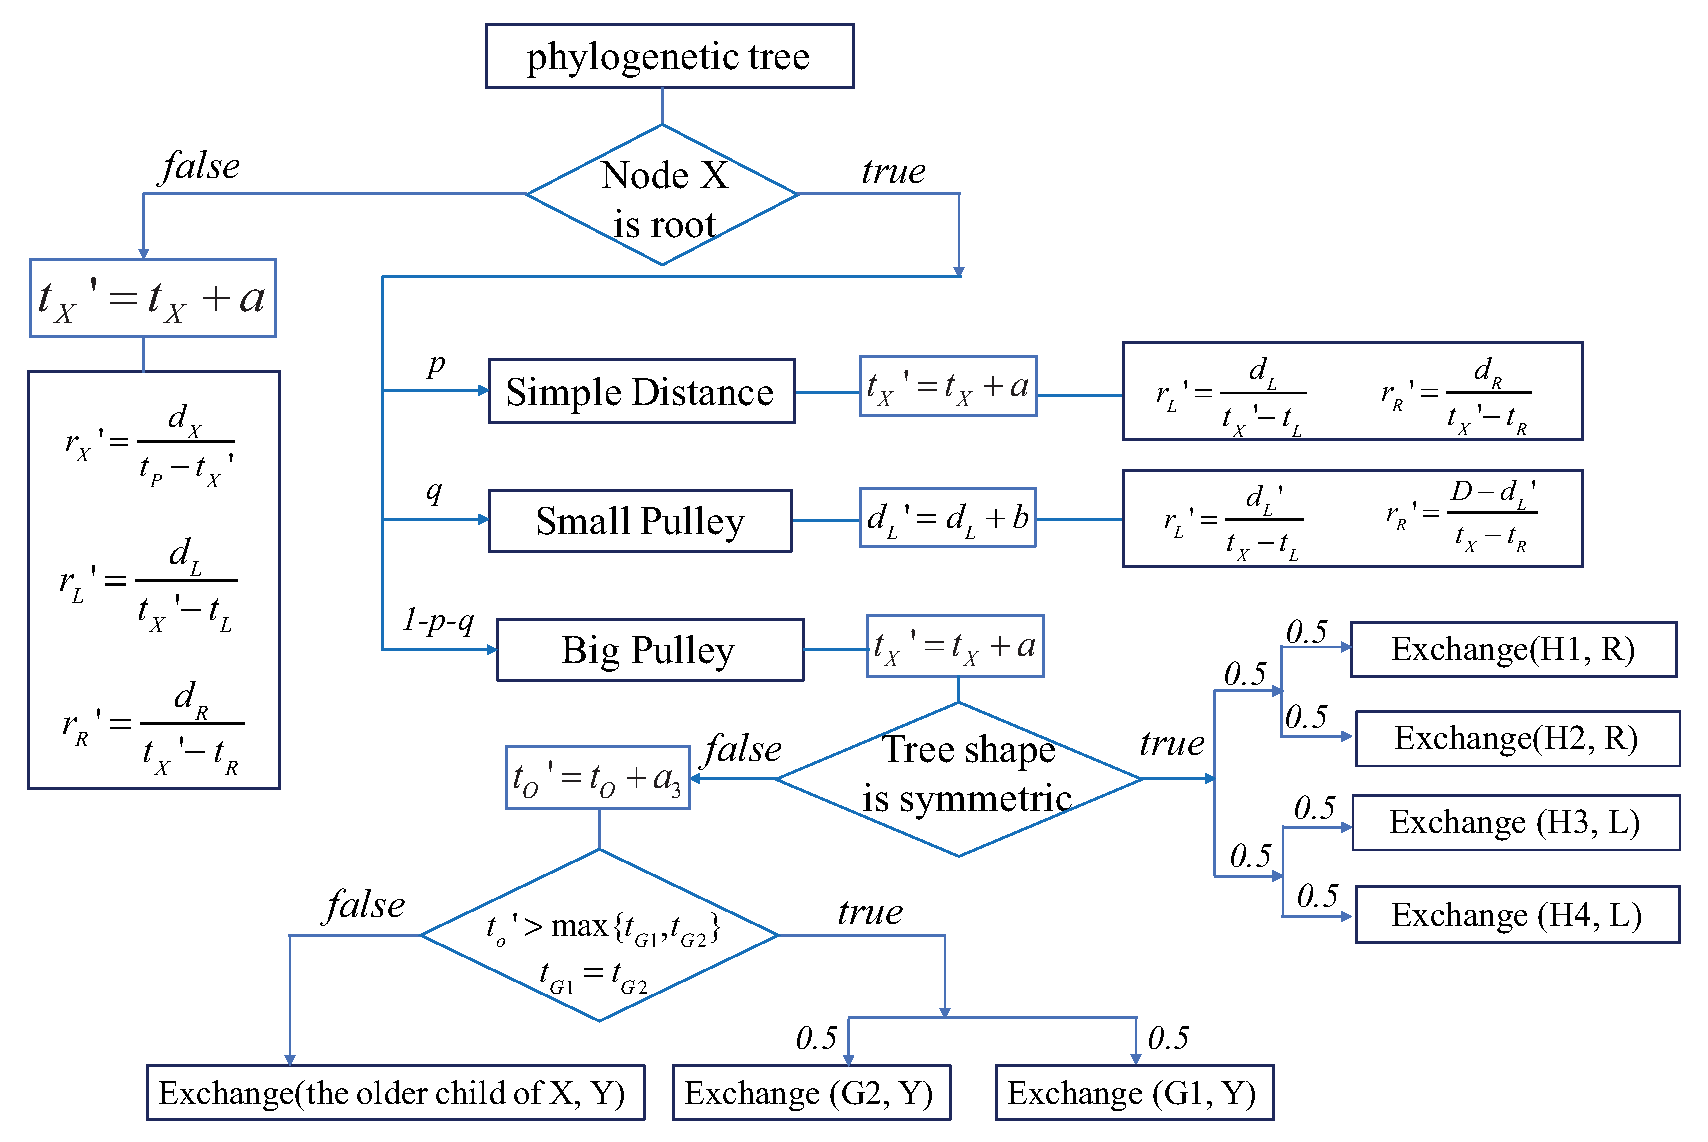
\includegraphics[width=12cm]{flowchart.eps}\\
\caption{\csentence{The flow chart of the constant distance operator.}
              }
\label{flowchart}
\end{figure}

\begin{figure}[h!]
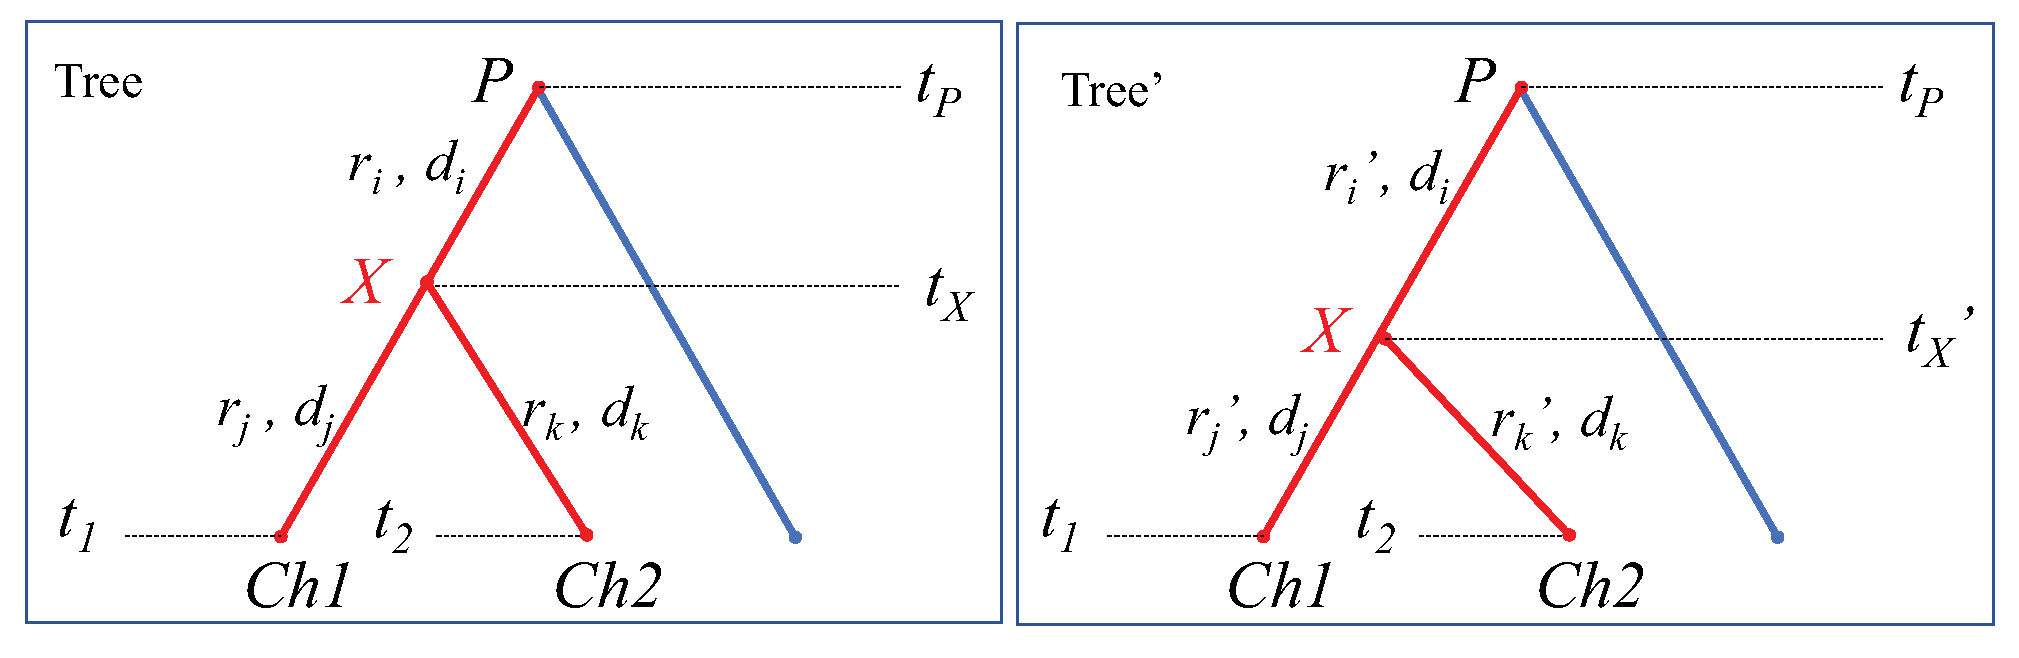
\includegraphics[width=12cm]{internalnodes.eps}\\
\caption{\csentence{The illustration of internal nodes.}
             }
\label{internalnodes}
\end{figure}

\begin{figure}[h!]
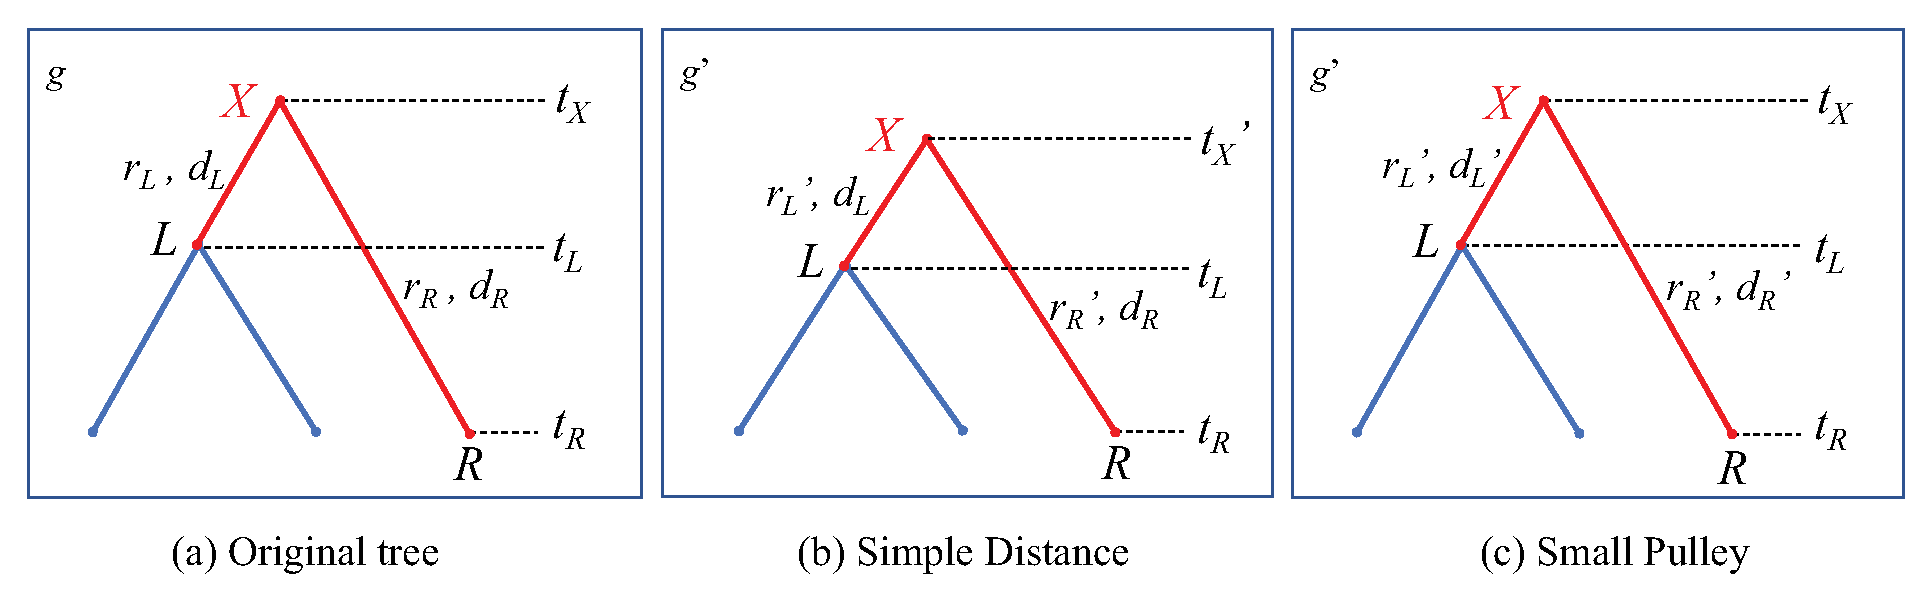
\includegraphics[width=12cm]{rootstrategy.eps}\\
\caption{\csentence{The illustration of root using simple distance.}
             }
\label{simpledistance}
\end{figure}


\begin{figure}[h!]
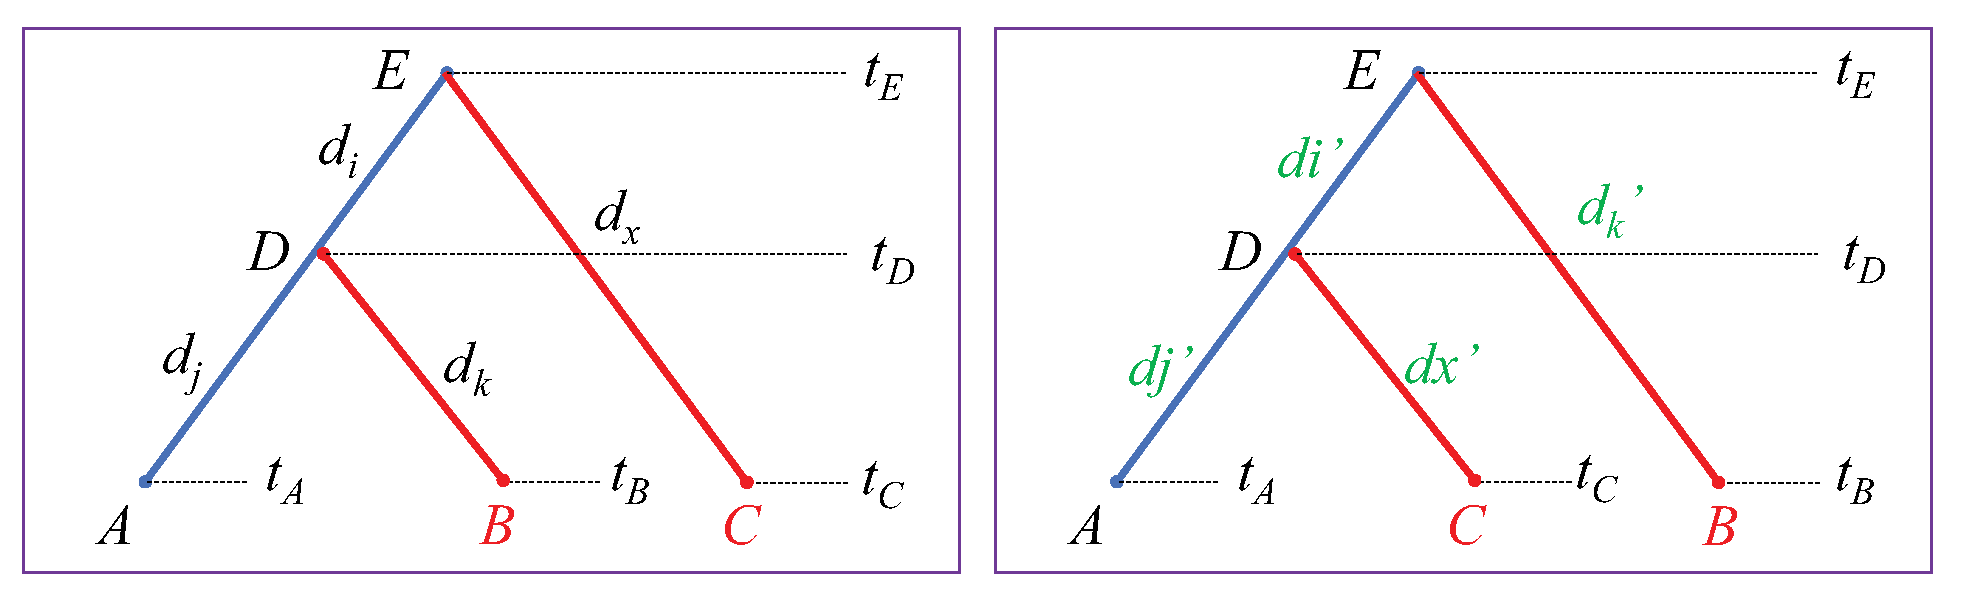
\includegraphics[width=12cm]{exchangemethod.eps}\\
\caption{\csentence{The illustration of \textit{Exchange (\textbf{B},\textbf{ C})} method.}
             }
\label{exchangemethod}
\end{figure}

\begin{figure}[h!]
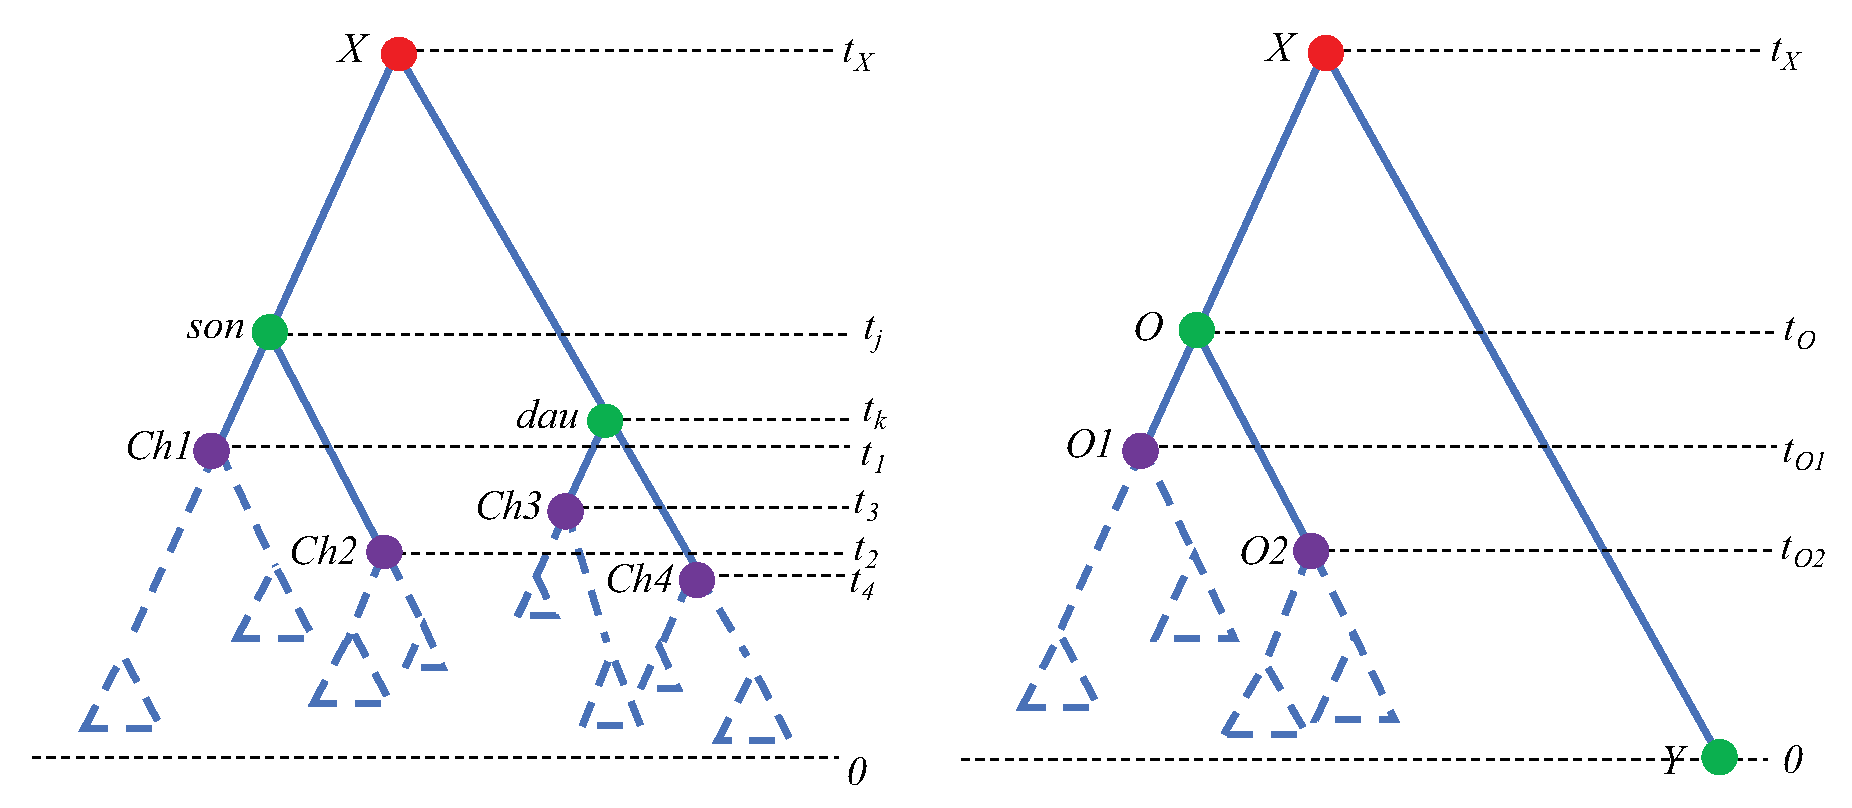
\includegraphics[width=12cm]{treeshape.eps}\\
\caption{\csentence{The illustration of tree shapes.}
             The symmetric tree is on the left and the asymmetric tree is on the right. The dashed triangles represent the potential subtrees rooted at the nodes.}
\label{treeshape}
\end{figure}

\begin{figure}[h!]
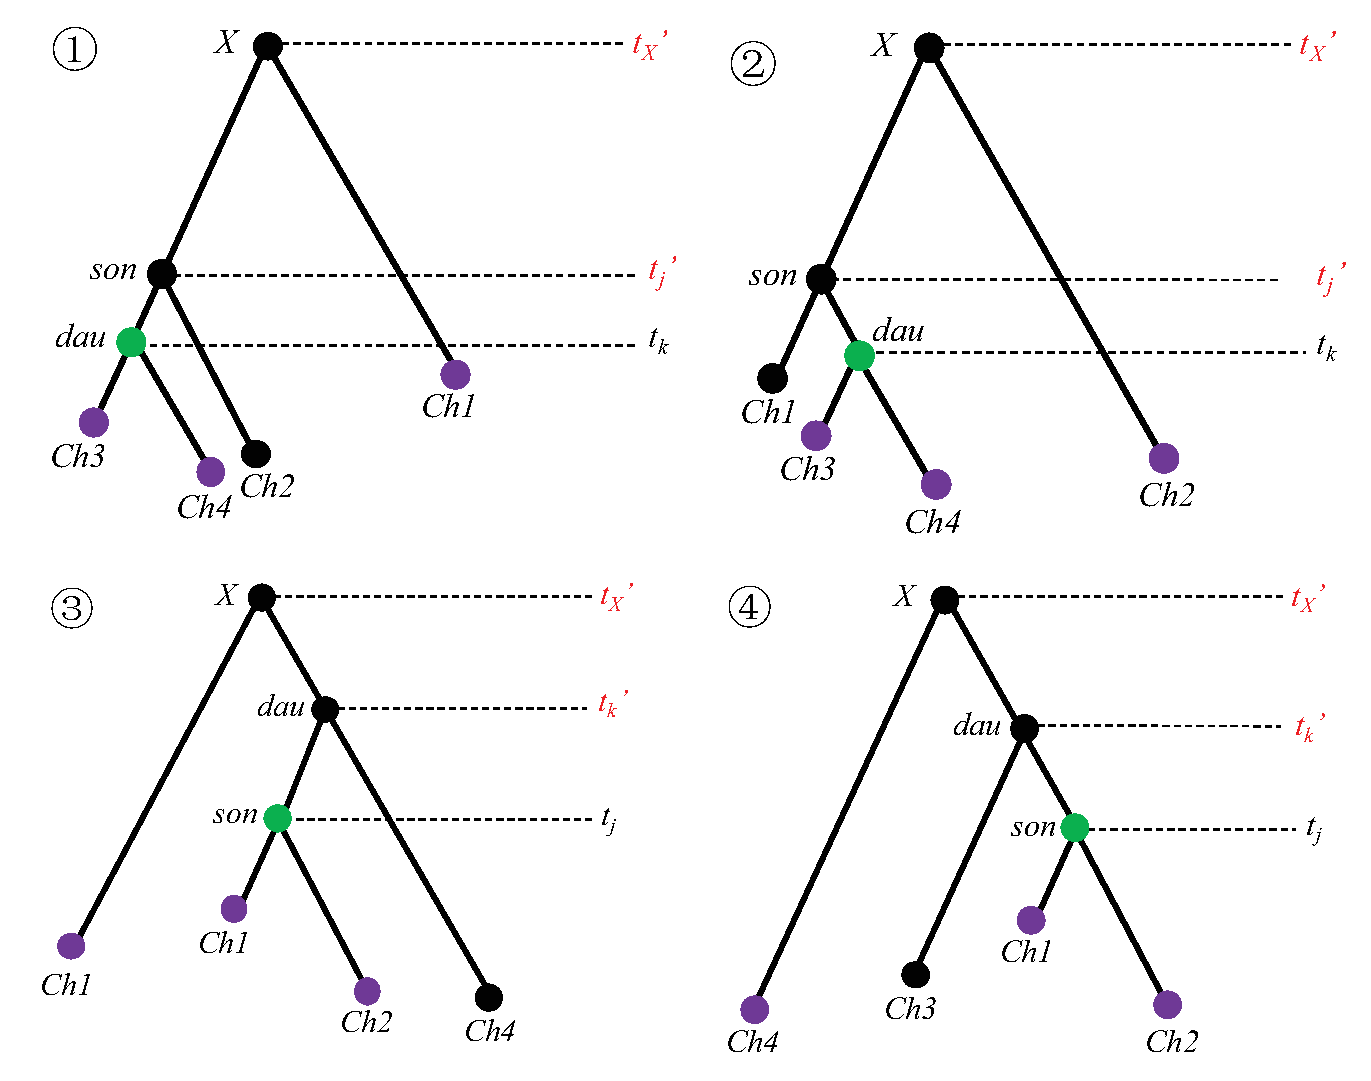
\includegraphics[width=12cm]{symmetric.eps}\\
\caption{\csentence{The illustration of symmetric trees.}
             }
\label{symmetric}
\end{figure}

\begin{figure}[h!]
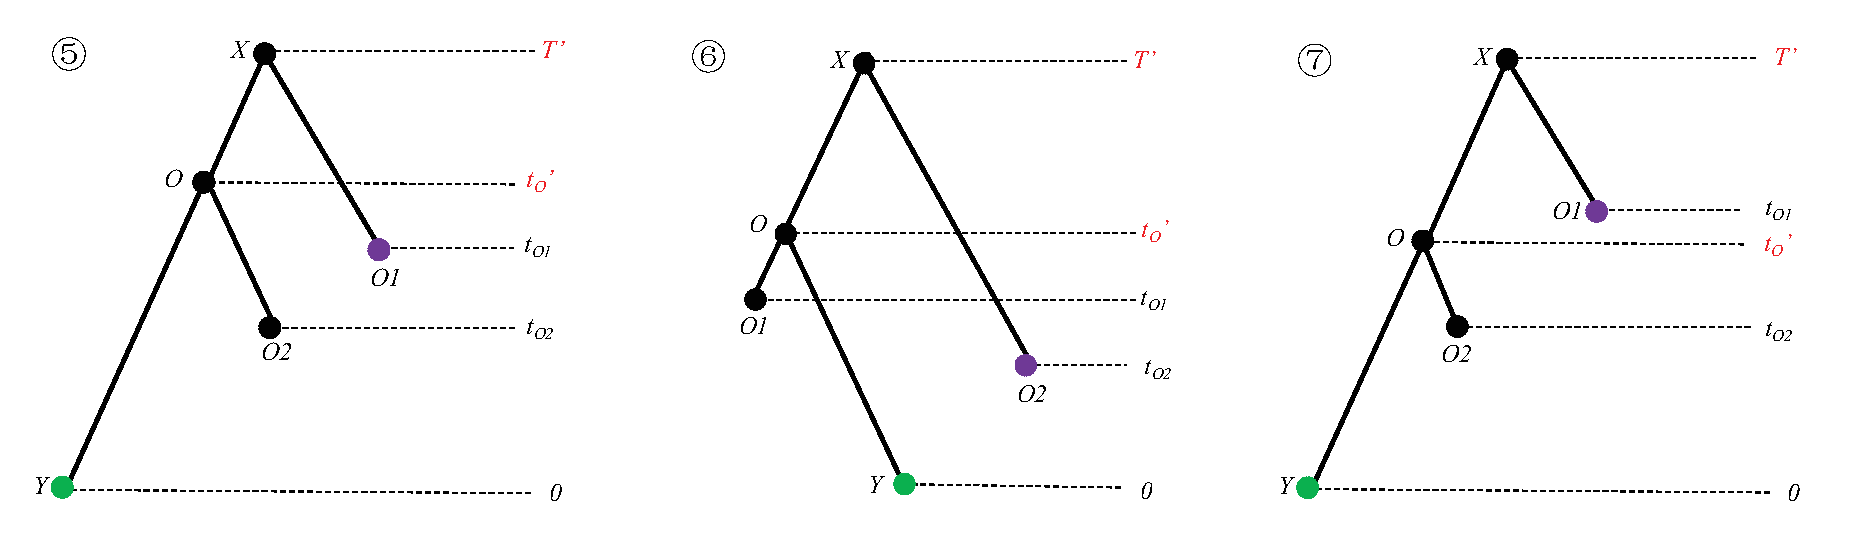
\includegraphics[width=12cm]{asymmetric.eps}\\
\caption{\csentence{The illustration of asymmetric trees.}
             }
\label{asymmetric}
\end{figure}

\begin{figure}[h!]
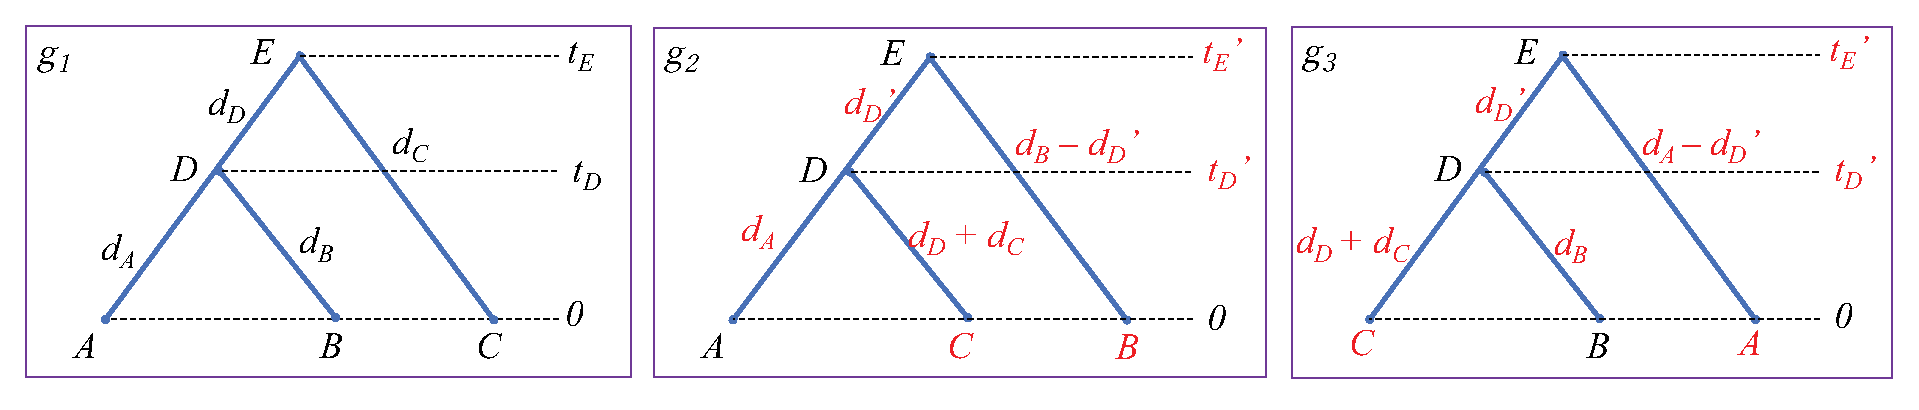
\includegraphics[width=12cm]{bigpulleyExp.eps}\\
\caption{\csentence{The illustration of sampling from prior.}
             }
\label{sampleprior}
\end{figure}

\begin{figure}[h!]
\centering
\subfigure[Senario 1: chain length = 10000000]{
\label{Fig.sub.1}
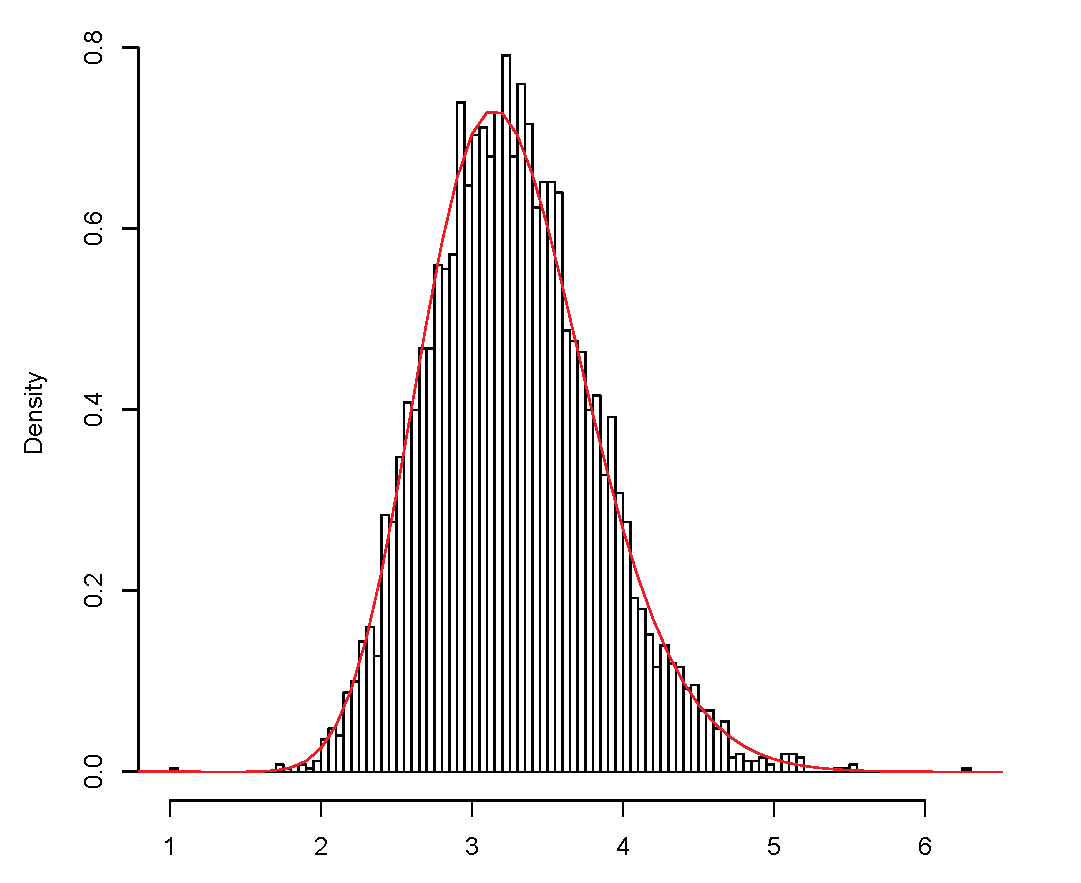
\includegraphics[width=0.45\textwidth]{Fig1}}
\subfigure[Senario 1: chain length = 20000000]{
\label{Fig.sub.2}
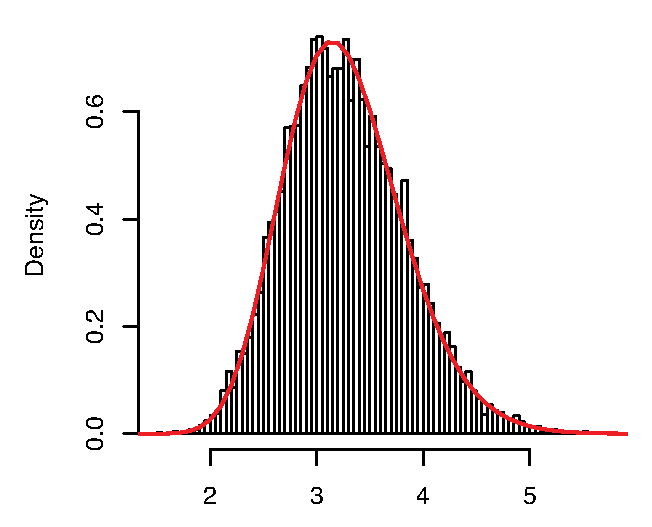
\includegraphics[width=0.45\textwidth]{Fig2}}
\subfigure[Senario 2: chain length = 10000000]{
\label{Fig.sub.3}
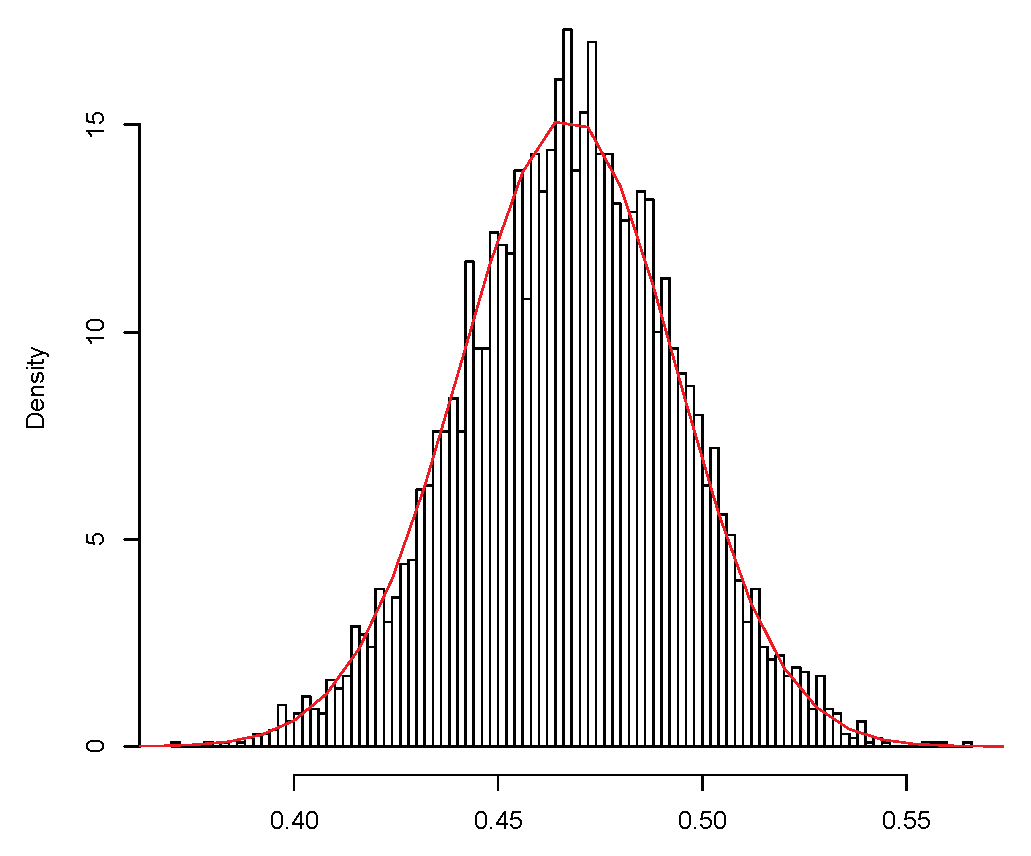
\includegraphics[width=0.45\textwidth]{Fig7}}
\subfigure[Senario 2: chain length = 20000000]{
\label{Fig.sub.4}
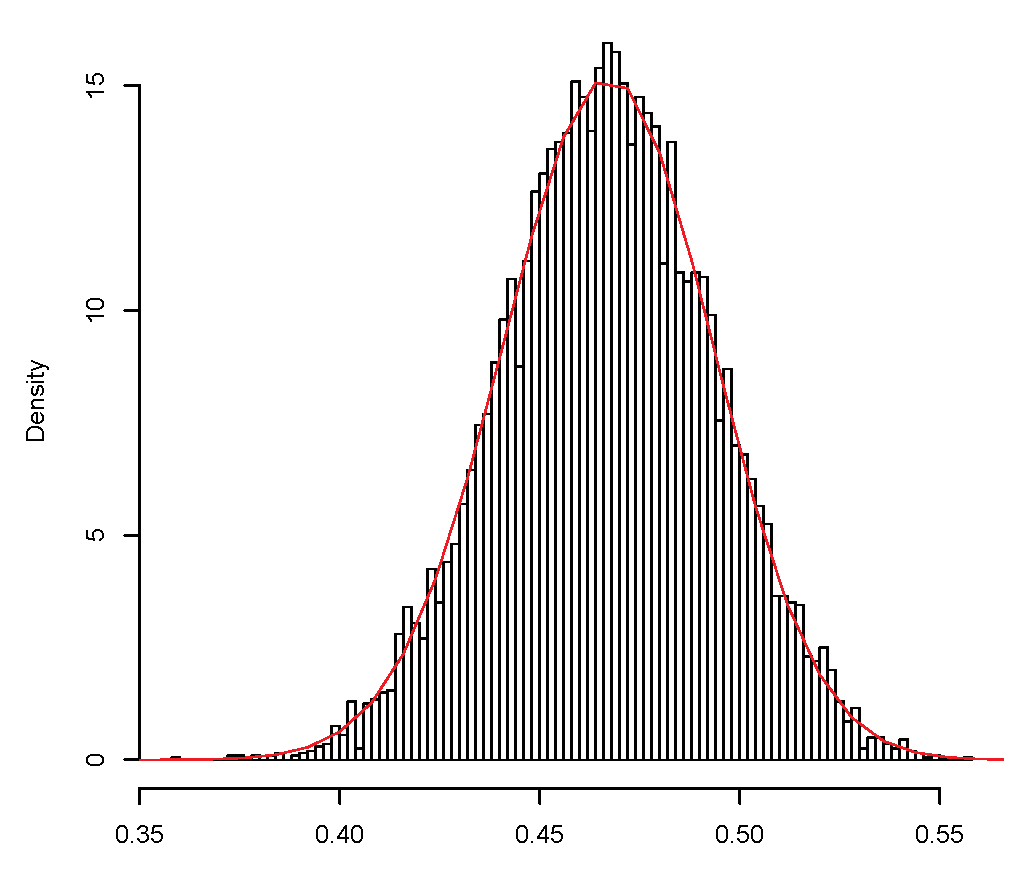
\includegraphics[width=0.45\textwidth]{Fig8}}
\caption{ Distributions of internal nodes}
\label{res_int}
\end{figure}

\begin{figure}[h!]
\centering
\subfigure[$t_E$ in Simple Distance]{
\label{Fig.sub.5}
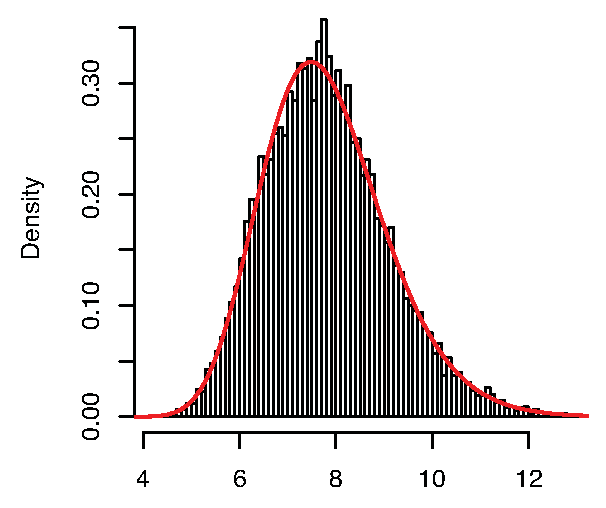
\includegraphics[width=0.35\textwidth]{RplotSD}}
\subfigure[$d_i$ in Small Pulley]{
\label{Fig.sub.6}
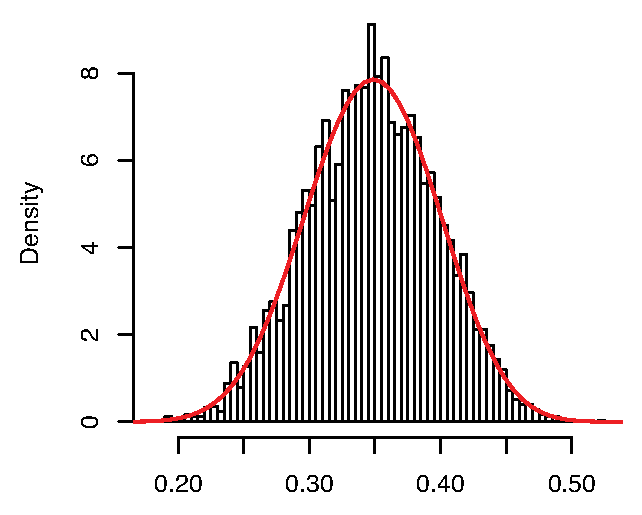
\includegraphics[width=0.35\textwidth]{RplotSP2}}
\subfigure[${d_i}$ in Big pulley]{
\label{Fig.sub.9}
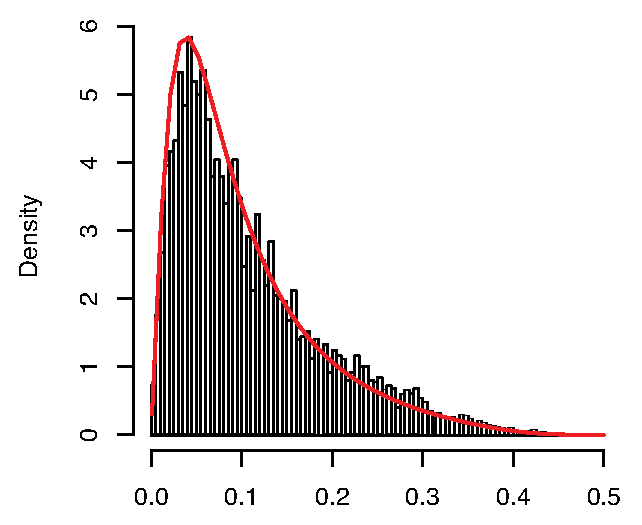
\includegraphics[width=0.35\textwidth]{bigd}}
\subfigure[${t_E}$ in Big pulley]{
\label{Fig.sub.10}
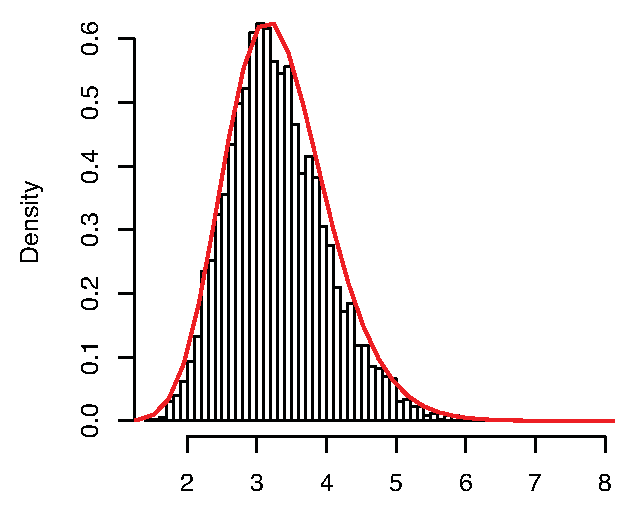
\includegraphics[width=0.35\textwidth]{bigT}}
\caption{Distributions of root}
\label{res_roo1}
\end{figure}

\begin{figure}[h!]
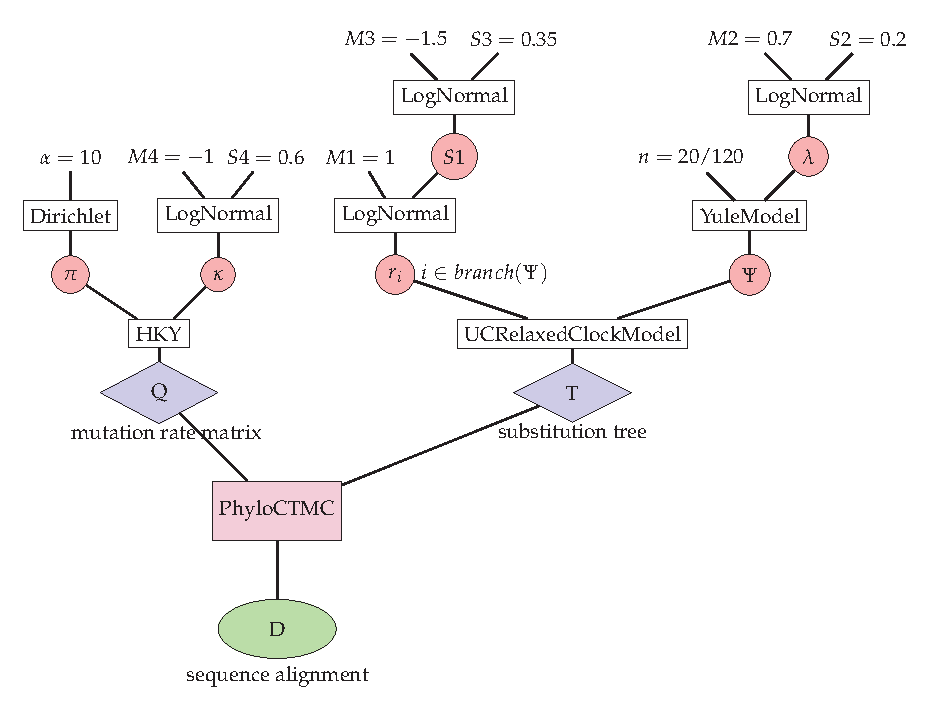
\includegraphics[width=12cm]{ModelValidation.eps}\\
\caption{\csentence{The models and prior distributions to simulate the sequence data.}
             }
\label{modelvalidation}
\end{figure}

\begin{figure}[h!]
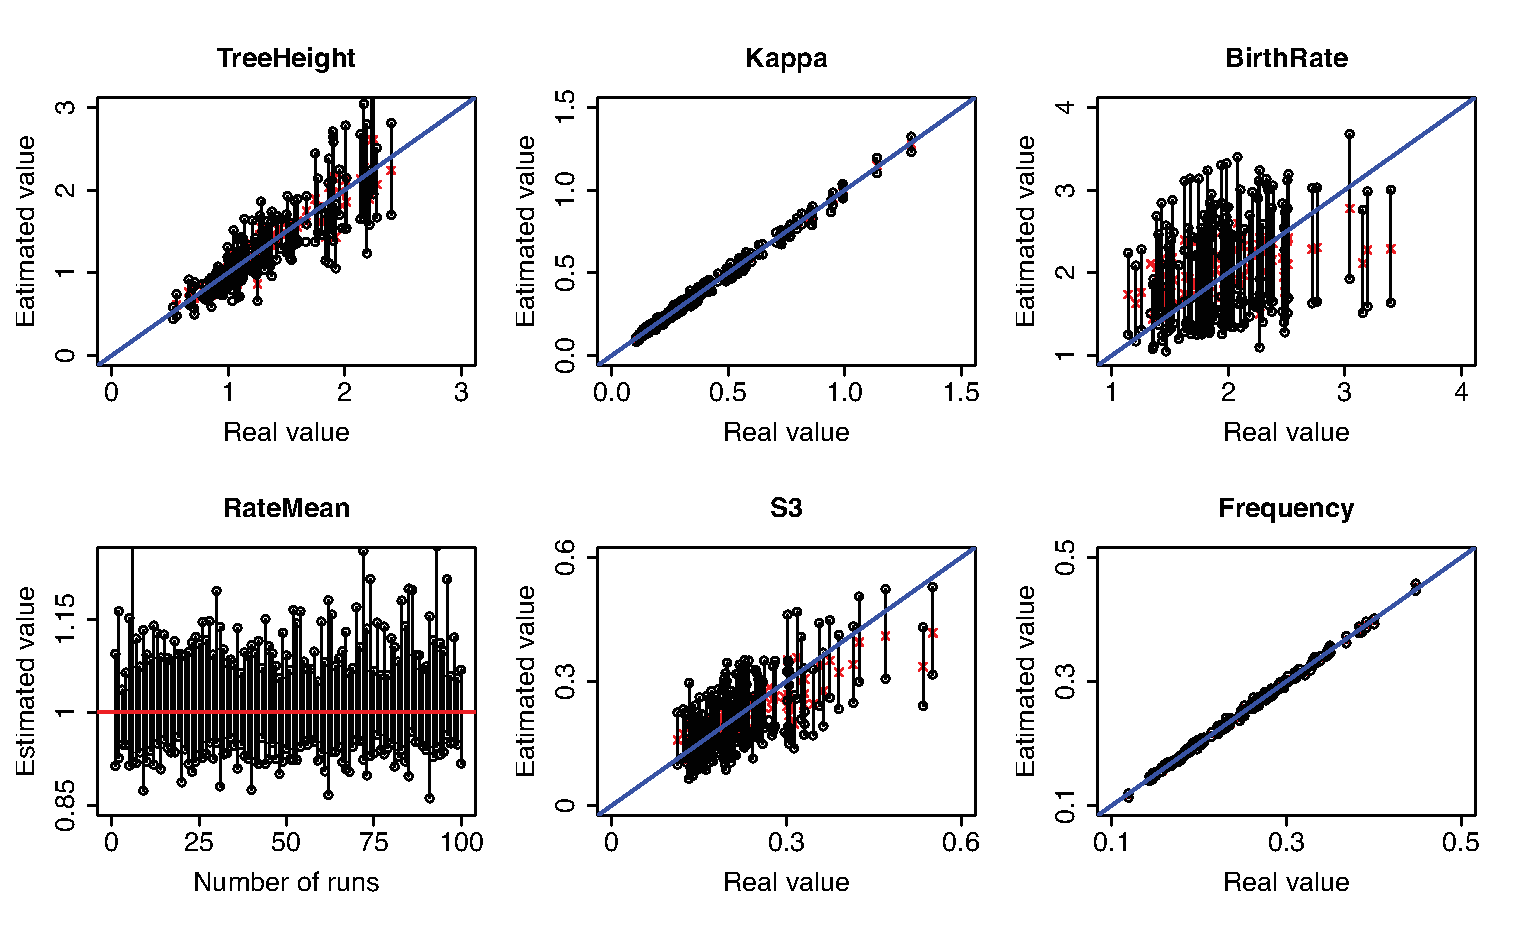
\includegraphics[width=12cm]{SmallTree.eps}\\
\caption{\csentence{Comparison of simulation study with 20 taxa.}
             }
\label{SmallTree}
\end{figure}

\begin{figure}[h!]
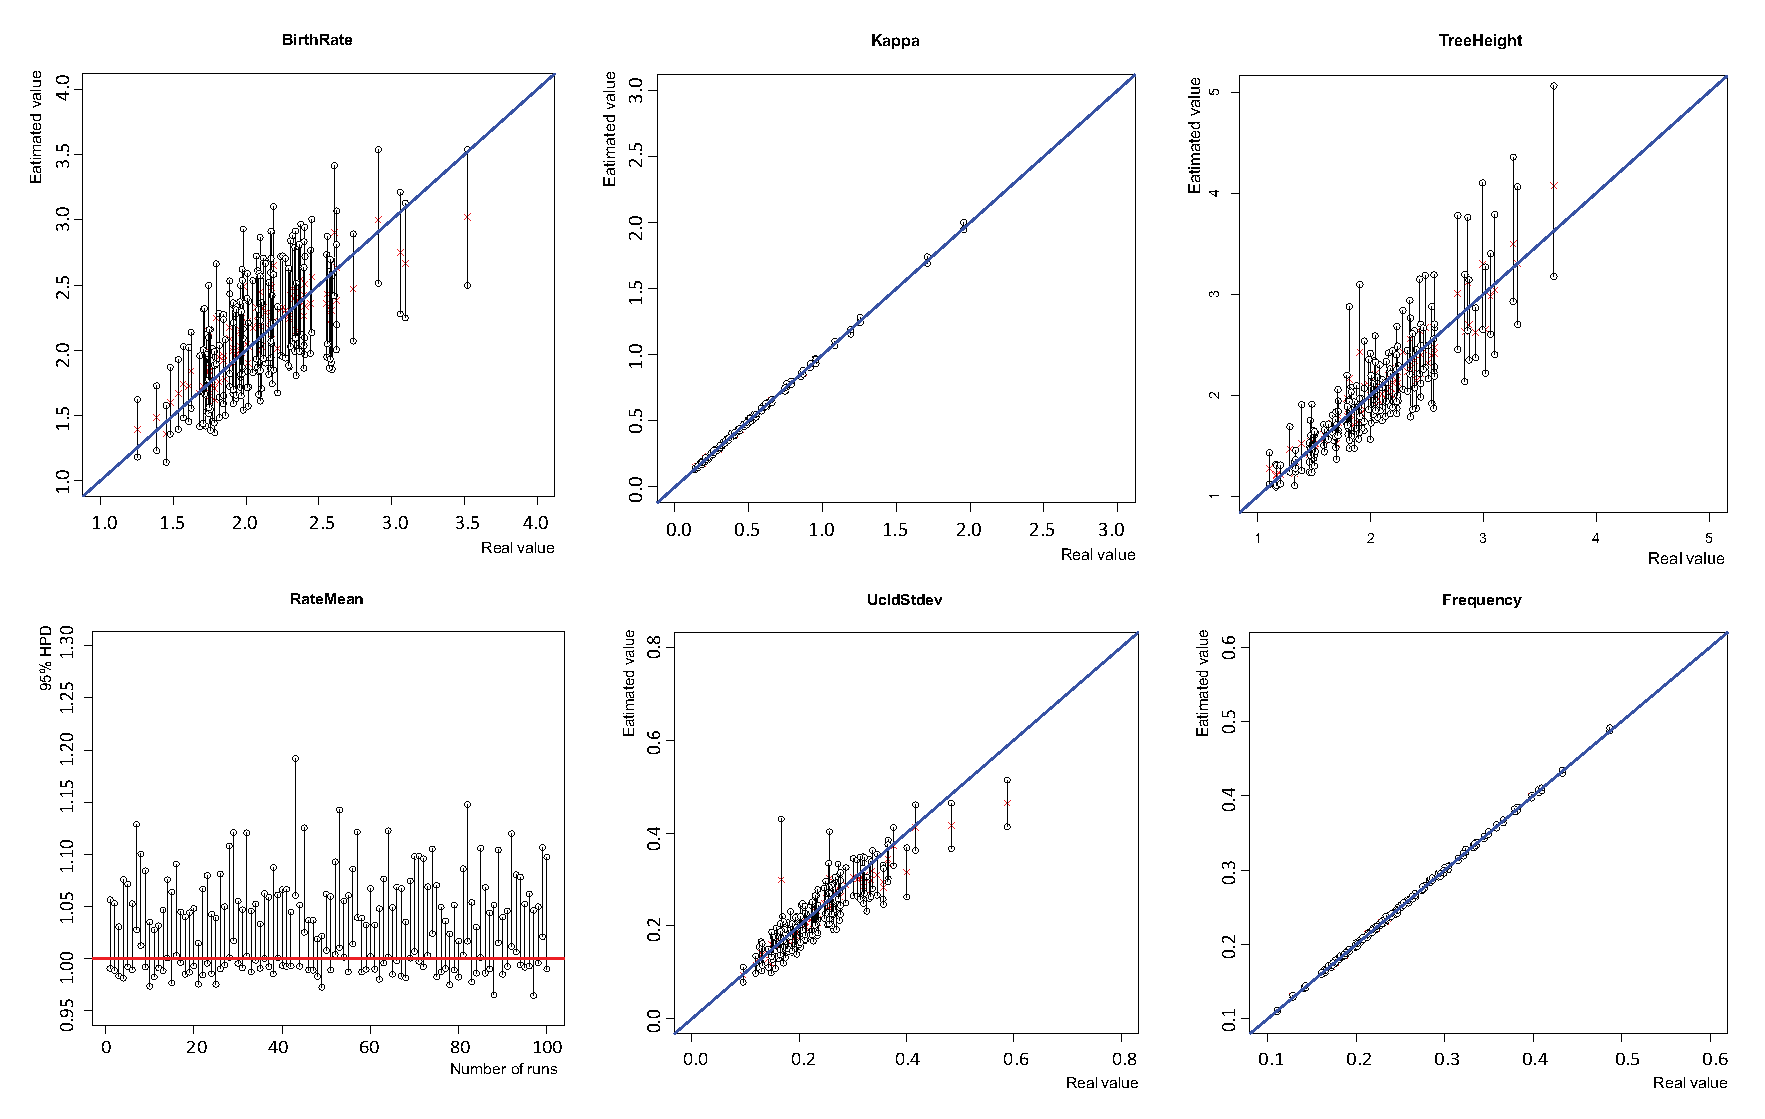
\includegraphics[width=12cm]{LargeTree.eps}\\
\caption{\csentence{Comparison of simulation study with 120 taxa.}
             }
\label{LargeTree}
\end{figure}

\begin{figure}[h!]
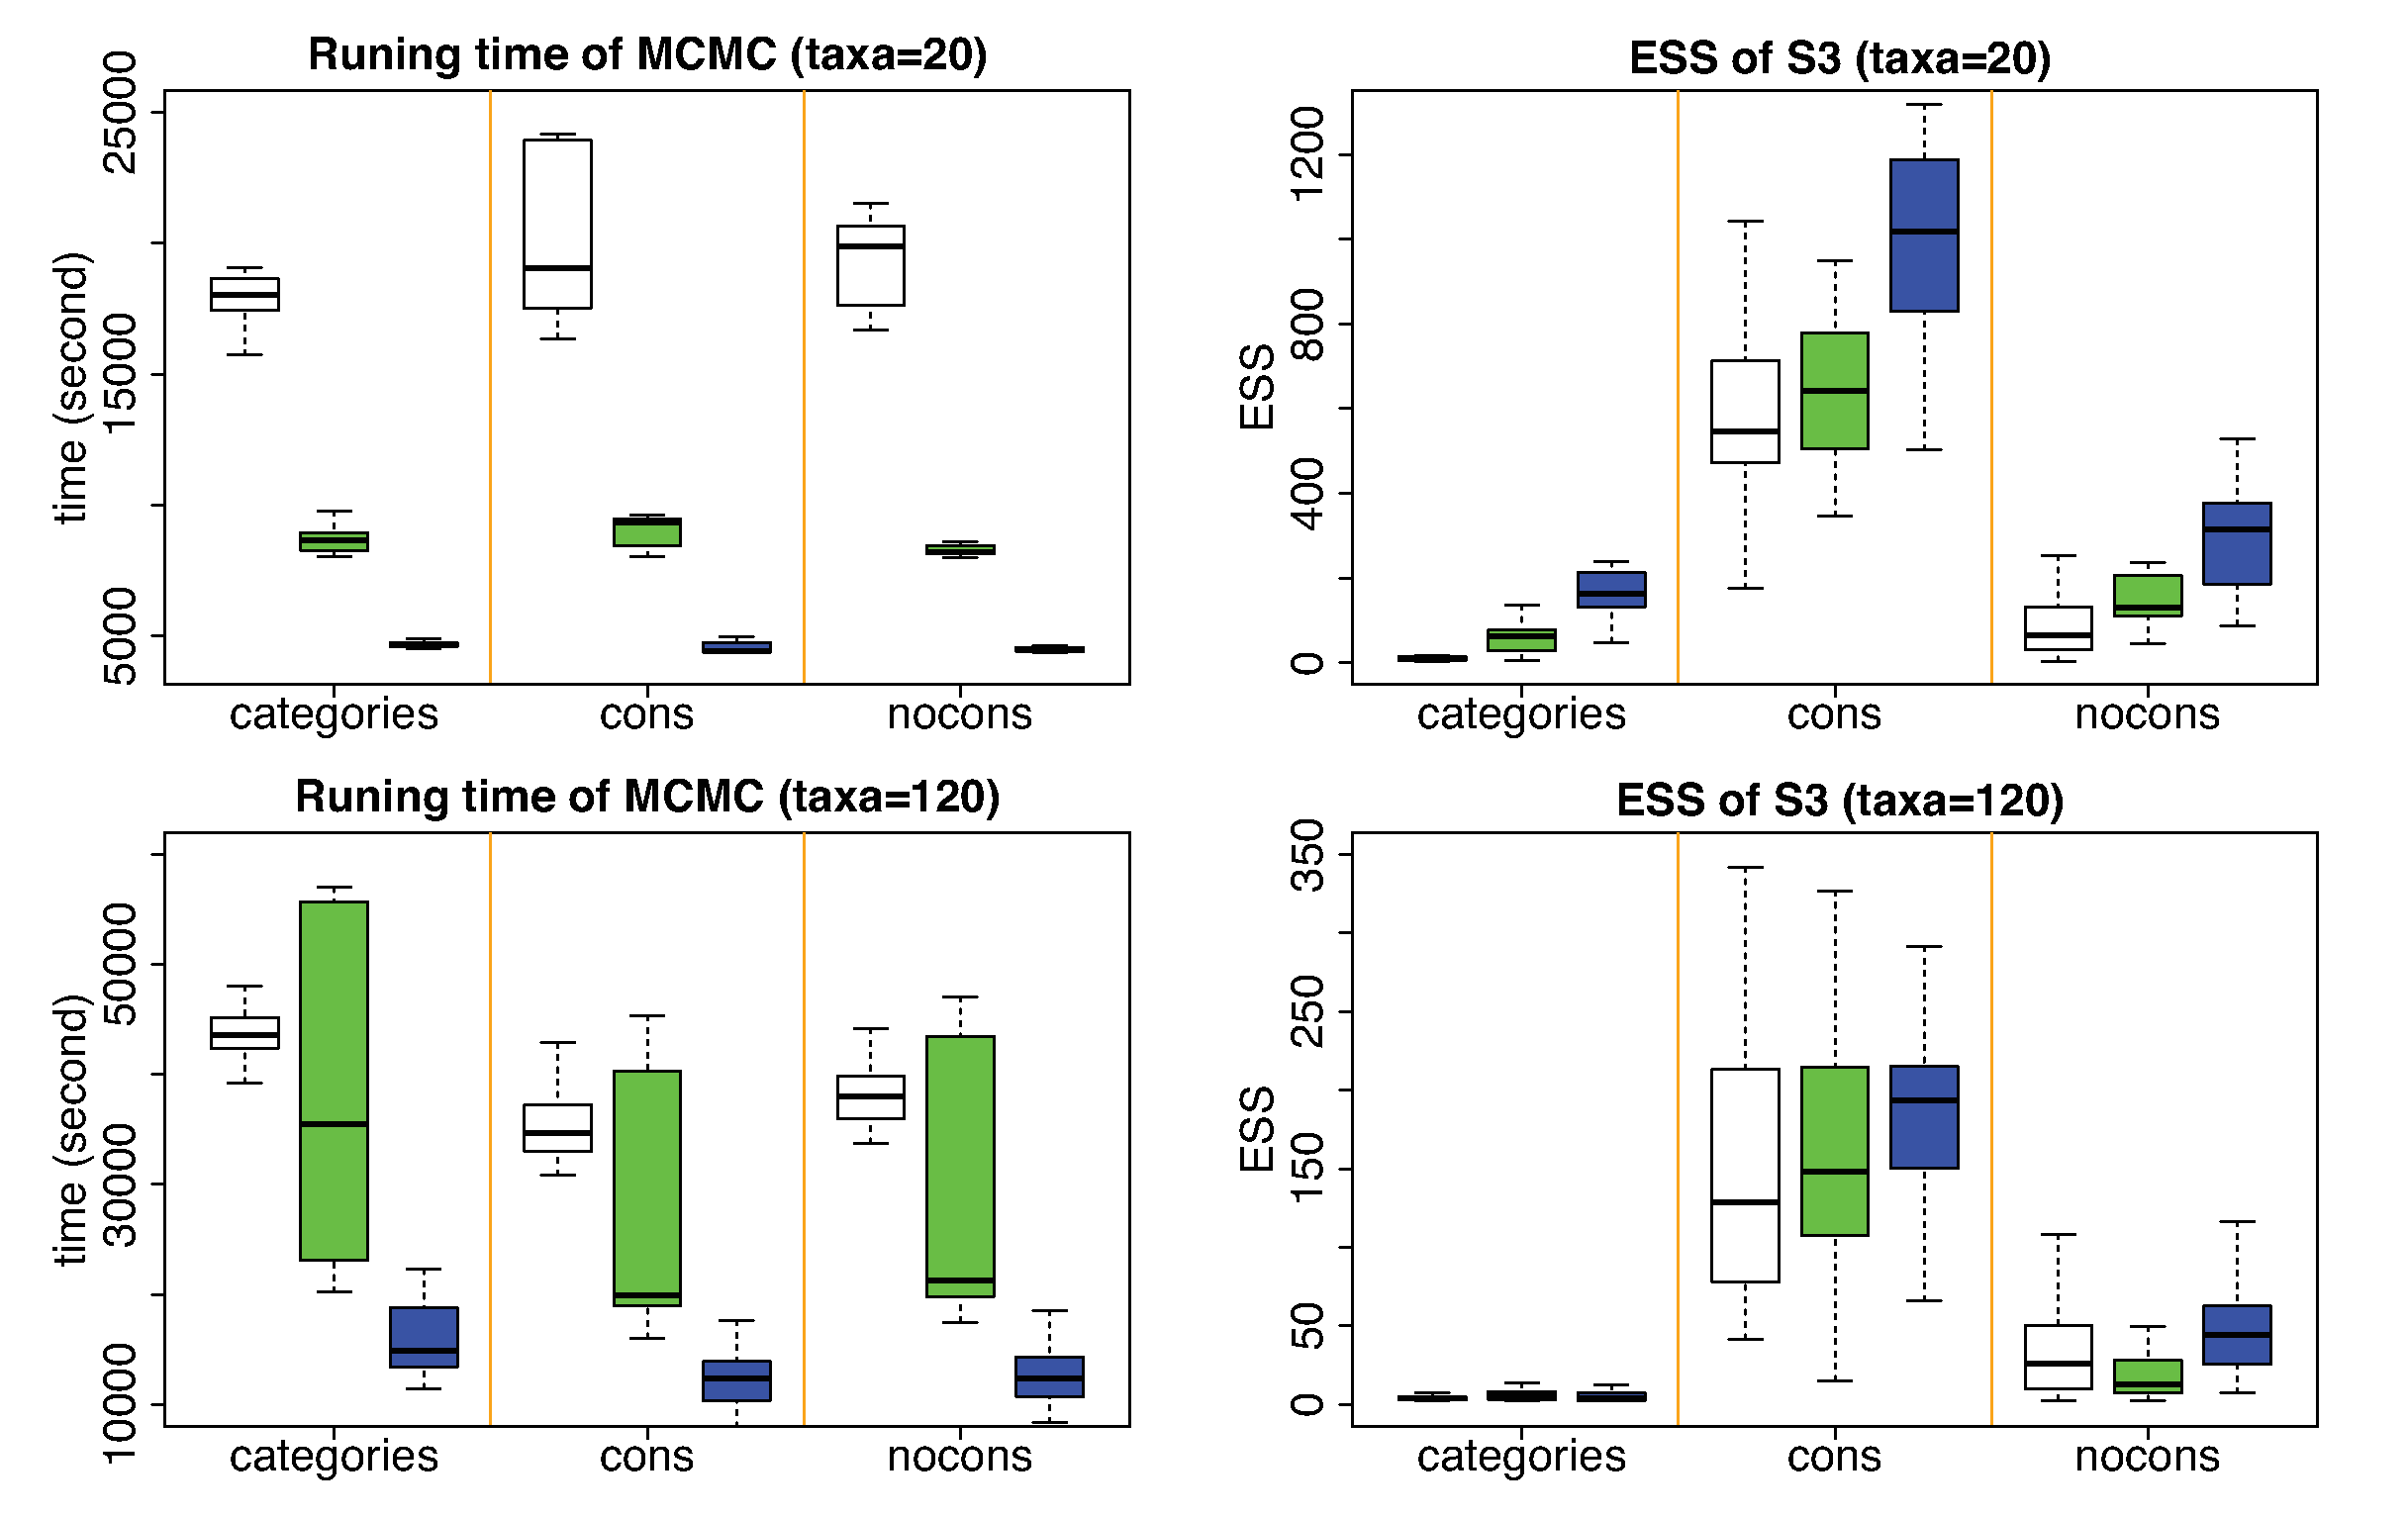
\includegraphics[width=12cm]{Efficiency.eps}\\
\caption{\csentence{Comparison of ESS and running time using simulated data.}
             }
\label{eff_comp}
\end{figure}

\begin{figure}[h!]
\centering
\subfigure{
\label{Fig.sub.1}
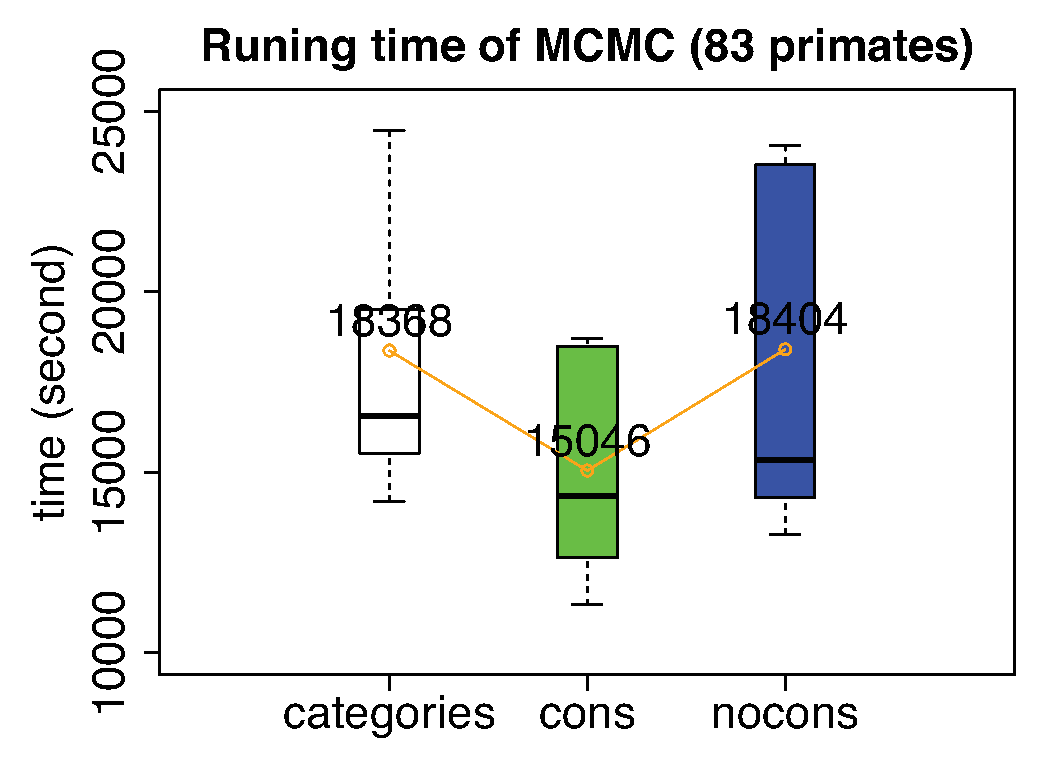
\includegraphics[width=0.5\textwidth]{primates1.eps}}
\subfigure{
\label{Fig.sub.2}
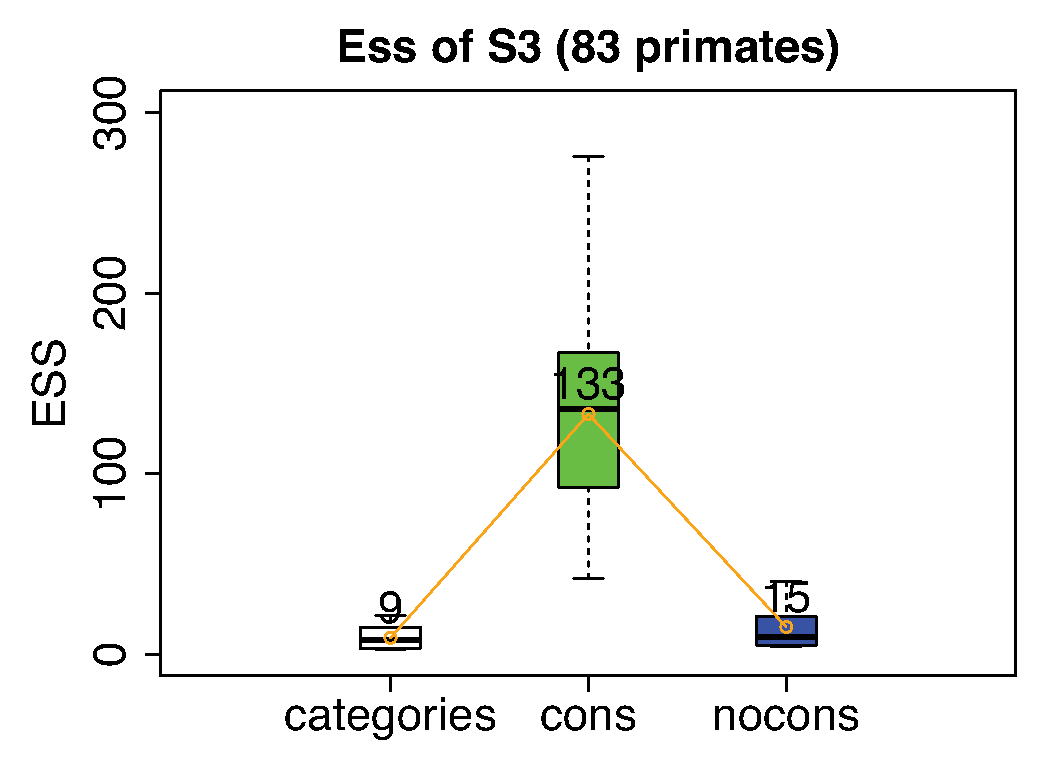
\includegraphics[width=0.5\textwidth]{primates2.eps}}
\caption{Comparison the ESS and ESS using primates data}
\label{eff_comp2}
\end{figure}
%%%%%%%%%%%%%%%%%%%%%%%%%%%%%%%%%%%
%%                               %%
%% Tables                        %%
%%                               %%
%%%%%%%%%%%%%%%%%%%%%%%%%%%%%%%%%%%
%% Use of \listoftables is discouraged.
%%
\section*{Tables}
\begin{table}[h!]
  \centering
\begin{tabular}{c|cccc|c|c|cccc}
  \hline
&\multicolumn{4}{c|}{genetic distances (fixed)}&$t_D$&$t_E$&\multicolumn{4}{c}{initial rates}\\
&${d_j}$&${d_k}$&${d_x}$&${d_i}$&initial&(fixed)&${r_j}$&${r_k}$&${r_x}$&${r_i}$\\
\hline
Scenario 1&0.1&0.2&0.4&0.27&1&10&0.1&0.2&0.04&0.03\\
\hline
Scenario 2&0.4&0.8&2.4&1.6&0.4&0.8&1&2&3&4\\
  \hline
\end{tabular}
\caption{Initial settings for internal nodes}\label{ini_inter}
\end{table}

\begin{table}[h!]
  \centering
\begin{tabular}{c|c|ccc|ccc|c}
  \hline
&\multirow{2}*{Chain Length}&\multicolumn{3}{c|}{Sample from MCMC}&\multicolumn{3}{c|}{R curve}&Plot\\
&~&Mean&Err&StdEv&Mean&Err&StdEv&\\
\hline
\multirow{2}*{Senario 1}&10000000&3.2727&8.3e-3&0.5467&\multirow{2}*{3.2669}&\multirow{2}*{1.3e-06}&\multirow{2}*{0.5553}&Fig.\ref{Fig.sub.1}\\
~&20000000&3.271&6.1e-3&0.5616&~&~&~&Fig.\ref{Fig.sub.2}\\
\hline
\multirow{2}*{Senario 2}&10000000&0.4677&3.9e-04&0.0265&\multirow{2}*{0.4667}&\multirow{2}*{3.5e-05}&\multirow{2}*{0.0262}&Fig.\ref{Fig.sub.3}\\
~&20000000&0.4672&2.8e-04&0.0262&~&~&~&Fig.\ref{Fig.sub.4}\\
  \hline
\end{tabular}
\caption{Results of internal nodes}\label{res_inter}
\end{table}

\begin{table}[h!]
  \centering
\begin{tabular}{c|cccc|c|c|cccc}
  \hline
\multirow{2}*{strategy}&\multicolumn{4}{c|}{genetic distances}&\multirow{2}*{$t_D$}&\multirow{2}*{$t_E$}&\multicolumn{4}{c}{initial rates}\\
~&${d_j}$&${d_k}$&${d_x}$&${d_i}$&~&~&${r_j}$&${r_k}$&${r_x}$&${r_i}$\\
\hline
Simple distance&0.1&0.2&0.4&0.27&1&10&0.1&0.2&0.04&0.03\\
Small pulley&0.1&0.2&\multicolumn{2}{|c|}{0.67}&1&10&0.1&0.2&0.04&0.03\\
Big pulley&0.5&0.5&\multicolumn{2}{|c|}{0.5}&5&10&0.1&0.1&0.03&0.04\\
  \hline
\end{tabular}
\caption{Initial settings for simple distance}\label{ini_sim}
\end{table}

\begin{table}[h!]
\centering
\begin{tabular}{c|c|cc|cc|cc}
  \hline
\multirow{2}*{Strategy}&\multirow{2}*{Variable}&\multicolumn{2}{c|}{Sample from MCMC}&\multicolumn{2}{c|}{R curve}&\multirow{2}*{Plot}\\
&~&Mean&StdEv&Mean&StdEv&\\
\hline
Simple distance&$t_E$&7.8081&1.2884&7.818691&1.299236&Fig.\ref{Fig.sub.5}\\
\hline
Small Pulley&${d_i}$&0.3480&0.0492&0.3476&0.0494&Fig.\ref{Fig.sub.6}\\
\hline
\multirow{2}*{Big Pulley}&${d_i}$&0.1016&0.0766&0.0960&0.0760&Fig.\ref{Fig.sub.9}\\
~&$t_E$&3.3017&0.6908&3.3095&0.6912&Fig.\ref{Fig.sub.10}\\
\hline
\end{tabular}
\caption{Results for root}\label{res_sma}
\end{table}

\begin{table}[h!]
  \centering
\begin{tabular}{cccccccc}
\hline
&BirthRate&TreeHeight&RateMean&UcldStdev&Kappa&Frequency\\
\hline
20 taxa&93&98&100&95&100&100\\
120 taxa&100&98&85&94&100&100\\
\hline
\end{tabular}
\caption{Number of real values lying in the 95\% HPD}\label{num_hpd}
\end{table}

\begin{table}[h!]
  \centering
\begin{tabular}{cc|cc|cc}
\hline
&&\multicolumn{2}{c|}{ESS}&\multicolumn{2}{c}{Running time}\\
\hline
&Length&20 taxa&120 taxa&20 taxa&120 taxa\\
categories&20000&12.80167&4.405382&18635&44155\\
&10000&57.99529667&6.316446&8660&36406\\
&5000&170.7803167&8.395184&4690&15956\\
Average&&80.52576111&6.372337333&10662&32172\\
\hline
cons&20000&615.8584&146.700042&20207&35406\\
&10000&645.72143&161.220762&8967&25589\\
&5000&993.1825567&186.265154&4581&12487\\
Average&&751.5874622&164.7286527&11252&24494\\
\hline
nocons&20000&86.46476333&62.77579&19344&38245\\
&10000&152.89205&19.598514&8361&30521\\
&5000&296.23683&47.514258&4499&12940\\
Average&&178.5312144&43.29618733&10735&27236\\
\hline
\end{tabular}
\caption{Results of ESS and running time}\label{eff_comp1}
\end{table}
%%%%%%%%%%%%%%%%%%%%%%%%%%%%%%%%%%%
%%                               %%
%% Additional Files              %%
%%                               %%
%%%%%%%%%%%%%%%%%%%%%%%%%%%%%%%%%%%

%\section*{Additional Files}
%  \subsection*{Additional file 1 --- Sample additional file title}
%    Additional file descriptions text (including details of how to
%    view the file, if it is in a non-standard format or the file extension).  This might
%    refer to a multi-page table or a figure.
%
%  \subsection*{Additional file 2 --- Sample additional file title}
%    Additional file descriptions text.


\end{backmatter}
\end{document}
